% ============================================================
% IEEE Conference Format
% A Reflexive Quantum-Kernel Intrusion Detection Approach
% Authors: Madhav Seth and Shiva Raj Pokhrel
% Deakin University / IIT Kharagpur, 2026
% ============================================================

\documentclass[conference]{IEEEtran}

% ---- Packages -----------------------------------------------
\usepackage{amsmath, amssymb, amsthm}
\usepackage{graphicx}
\usepackage{booktabs}
\usepackage{multirow}
\usepackage{array}
\usepackage[hidelinks]{hyperref}
\usepackage{xcolor}
\usepackage{algorithm}
\usepackage{algorithmic}
\usepackage{cite}
\usepackage{url}
\usepackage{pifont}

\setlength{\heavyrulewidth}{0.08em}
\setlength{\lightrulewidth}{0.05em}

\newtheorem{proposition}{Proposition}

% ============================================================
\begin{document}

\title{A Reflexive Quantum-Kernel Intrusion Detection Approach}

\author{
\IEEEauthorblockN{Madhav Seth}
\IEEEauthorblockA{Indian Institute of Technology, Kharagpur\\
Kharagpur, India}
\and
\IEEEauthorblockN{Shiva Raj Pokhrel, \textit{Senior Member, IEEE}}
\IEEEauthorblockA{School of Information Technology\\
Deakin University, Australia}
}

\maketitle

% ---- Abstract -----------------------------------------------
\begin{abstract}
Network intrusion detectors trained on one deployment can degrade sharply
when traffic statistics, attack mechanisms, or class priors change across
networks. This paper presents \textbf{Q-ARMOR}, a stateful
quantum--classical intrusion-detection architecture that couples an
8-qubit fidelity quantum kernel with episodic performance monitoring and
targeted cross-domain adaptation. The data plane uses a
Detect$\to$Type cascade: PegasosQSVC performs binary attack detection and
a classical Random Forest performs coarse attack typing. The control plane
maintains episodic memory and applies explicit adaptation actions when
detector performance and drift evidence indicate that the current
operating regime is no longer adequate. Unlike reinforcement-learning
claims, the present controller is formulated conservatively as a
deterministic reflexive policy whose state persists across episodes. We
evaluate Q-Armor on NF-ToN-IoT (1.38M flows) and NF-UNSW-NB15 (1.62M
flows). Within-domain AUROC reaches \textbf{0.973} with macro-F1
\textbf{0.496}; cross-domain AUROC drops to \textbf{0.606} and recovers to
\textbf{0.913} after retraining on 150 target samples. We also formalise
fidelity-kernel PSD properties, finite-shot concentration, and adaptation
assumptions, and we report a preliminary pilot in which the deterministic
reflector is replaced by an LLM-gated inference-time decision function
guarded by a deterministic verifier -- explicitly \emph{not} a
reinforcement-learning extension. The results support quantum-kernel
adaptation as a compact representation study, not a claim of quantum
advantage.
\end{abstract}

\begin{IEEEkeywords}
network intrusion detection, quantum machine learning, quantum kernel,
domain shift, concept drift, adaptive security, episodic memory, IoT
security, large language model agents
\end{IEEEkeywords}

% ============================================================
\section{Introduction}
\label{sec:introduction}
% ============================================================

Network intrusion detection is intrinsically non-stationary. A detector
trained on one network may encounter different protocol mixtures, service
profiles, traffic volumes, attack families, and class priors after
deployment. Consequently, strong within-dataset accuracy does not by
itself establish operational robustness. The central question studied
here is therefore not whether a quantum classifier can fit one
intrusion-detection dataset, but whether a compact quantum-kernel detector
can be \emph{monitored and selectively adapted} when its deployment
distribution changes.

Quantum kernel methods provide a useful representation-learning testbed
because classical flow vectors are embedded into quantum states and
compared through state overlap \cite{havlicek2019, schuld2019}. However,
such models also face important limitations: kernel estimation scales
quadratically with training-set size, finite shots perturb Gram matrices,
noise can collapse useful kernel variation, and classical models may match
quantum prediction once sufficient labelled data are available
\cite{huang2021, cerezo2022, thanasilp2024}. We therefore make no quantum
speedup or quantum-advantage claim. Instead, the quantum component is
studied as a small-sample representation and adaptation mechanism embedded
inside a larger security control loop.

A second challenge is terminology. A controller that records outcomes and
executes hand-designed rules is stateful and autonomous, but it is not
automatically a learned policy. The original prototype was inspired by the
actor--evaluator--memory structure of Reflexion \cite{shinn2023}; the
revised formulation therefore uses the more precise term \emph{reflexive
episodic control}. The current controller stores performance episodes,
selects actions from a finite intervention set, and persists state, but
its action logic remains deterministic. This distinction is important for
reproducibility and for separating demonstrated capability from future
meta-learning extensions -- including the LLM-gated pilot introduced in
Section~\ref{subsec:llm_pilot}, which is likewise not a learned policy.

\subsection{Research Questions}

We organise the study around four research questions.

\begin{enumerate}
\item \textbf{Within-domain utility.} Can a small, balanced quantum-kernel
subset provide useful binary attack discrimination on held-out traffic?
\item \textbf{Cross-domain robustness.} How severely does performance
degrade when the source-trained detector is transferred to a
heterogeneous target network?
\item \textbf{Target-budget adaptation.} Can representative reselection of
a small labelled target subset recover part of the lost binary detection
performance?
\item \textbf{Reflexive control.} Can persistent episodic state
distinguish between a degradation event requiring model switching and one
requiring target-domain retraining under the present supervised-feedback
assumptions?
\end{enumerate}

\subsection{Contributions}

The paper makes the following contributions.

\begin{enumerate}
\item We formulate Q-ARMOR as a two-plane adaptive IDS: a
quantum--classical Detect$\to$Type data plane and a persistent episodic
control plane. The revision explicitly distinguishes deterministic
reflexive control from reinforcement or policy learning.
\item We define an 8-qubit \textit{CyberSecurityFeatureMap} and fidelity
kernel for NetFlow features and state the exact positive-semidefinite
property of the ideal kernel. We additionally derive a finite-shot
entry-wise error bound that links quantum measurement budget to
kernel-estimation accuracy.
\item We introduce \textsc{Switch-Subset}, a target-budget adaptation
mechanism that reselects a representative balanced target subset and
retrains the binary quantum-kernel detector without retraining on the
full target dataset.
\item We provide cross-domain evidence on NF-ToN-IoT and NF-UNSW-NB15 and
explicitly separate observed domain shift from the stronger concept-drift
claim. The current results show a binary AUROC recovery of $+0.307$ after
target-subset adaptation, while also showing that attack typing does not
transfer.
\item We define a publication-grade validation protocol covering score
orientation, leakage control, equal target-label budgets, natural class
prevalence, repeated seeds, calibration, kernel geometry, finite-shot
noise, and intervention cost, and we run it: Sections~\ref{subsec:audit_status}--\ref{subsec:confirmatory}
and~\ref{subsec:budgetsweep}--\ref{subsec:recurpoison} report, honestly,
which parts the present study satisfies and which remain open.
\item We report a preliminary pilot in which the heuristic reflector is
replaced by a four-stage LLM-gated decision function (Diagnoser, Planner,
deterministic Verifier, Reflector) as an alternative, \emph{not learned},
reflexive controller, and compare it against the heuristic baseline under
identical episode conditions (Section~\ref{subsec:llm_pilot}).
\end{enumerate}

% ============================================================
\section{Related Work \& Q-Armor}
\label{sec:related}
% ============================================================

\subsection{Intrusion Detection under Distribution Shift}

Classical intrusion detection spans tree ensembles, kernel methods, deep
neural networks, and representation-learning approaches \cite{liao2013}.
Random Forests remain strong baselines for tabular flow data because they
capture nonlinear interactions without requiring feature standardisation
\cite{breiman2001}. A persistent weakness in IDS evaluation is that train
and test data are often drawn from the same corpus, even though deployment
occurs under a different traffic distribution. Domain-adaptation theory
makes this distinction explicit: target risk depends on both source error
and divergence between source and target distributions \cite{bendavid2010}.
We therefore treat NF-ToN-IoT $\to$ NF-UNSW-NB15 as a cross-domain
transfer problem rather than assuming that every cross-dataset change is a
concept drift.

\subsection{Quantum Kernels and Quantum Machine Learning}

Quantum feature maps embed classical vectors into quantum states and use
state overlap as a kernel for a classical convex learner
\cite{havlicek2019, schuld2019}. The appeal is representational rather
than automatically computational: an expressive Hilbert-space map may
generate geometry that differs from conventional classical kernels.
However, Huang et al. showed that classical learners can often reproduce
useful predictive structure once data are available, motivating explicit
classical--quantum geometric comparisons \cite{huang2021}. More recently,
Thanasilp et al. established that fidelity kernels can exhibit exponential
concentration due to embedding expressivity, global measurements,
entanglement, or noise \cite{thanasilp2024}. These results motivate
shallow, problem-inspired embeddings, finite-shot sensitivity analysis,
and conservative claims.

Quantum intrusion-detection studies remain relatively immature compared
with classical IDS literature. Existing work has explored quantum
classification and hybrid models for security data \cite{kalinin2022};
nevertheless, many studies use small balanced samples, ideal simulation,
or within-dataset evaluation. Q-ARMOR therefore focuses specifically on
the interaction between compact quantum-kernel learning and cross-domain
adaptation.

\subsection{Drift Detection and Reflexive Agents}

ADWIN detects statistically significant changes in a monitored stream
using adaptive windows \cite{bifet2007}. When it is fed prediction errors,
labels are required; this is an important deployment assumption rather
than a label-free drift solution. Separately, Reflexion introduced
episodic self-evaluation and memory for language agents \cite{shinn2023}.
Q-ARMOR borrows the architectural pattern of actor, evaluator, memory, and
revised action, but uses typed numerical interventions rather than
natural-language self-critique. The current version therefore constitutes
a \emph{reflexive controller}; learning the intervention policy itself is
left to a future contextual-bandit or reinforcement-learning extension. A
second, LLM-gated variant of the reflector is piloted in
Section~\ref{subsec:llm_pilot}; it substitutes natural-language reasoning
for the four hand-coded rules but, like the rule-based controller, updates
no parameters from experience and therefore does not constitute policy
learning either.

\subsection{Originality and Novelty of Q-ARMOR}

Figure~\ref{fig:overview} presents the originality and novelty of Q-ARMOR
as a reflexive, hybrid intrusion-detection architecture designed for
cross-domain network security adaptation. The system is organised into two
tightly coupled components: an inner detection pipeline and an outer
adaptation loop. The inner pipeline begins with NetFlow feature
preprocessing, followed by an 8-qubit \textit{CyberSecurityFeatureMap}
that embeds traffic features into a quantum feature space. A fidelity
quantum kernel is then constructed and used by PegasosQSVC for Stage~1
binary attack detection. Samples classified as benign terminate at this
stage, whereas predicted attacks are forwarded to a Stage~2 classical
Random Forest typer for coarse attack categorisation, including DoS,
Injection, Recon, and Backdoor. The source-to-target transition from
NF-ToN-IoT to NF-UNSW-NB15 explicitly represents the cross-domain setting,
where substantial differences in traffic distributions and attack
taxonomies introduce severe deployment shift. Thus, Q-Armor is formulated
not as a static classifier, but as a structured framework for quantum
representation, intrusion detection, and adaptive response under network
domain shift.

\begin{figure*}[t]
\centering
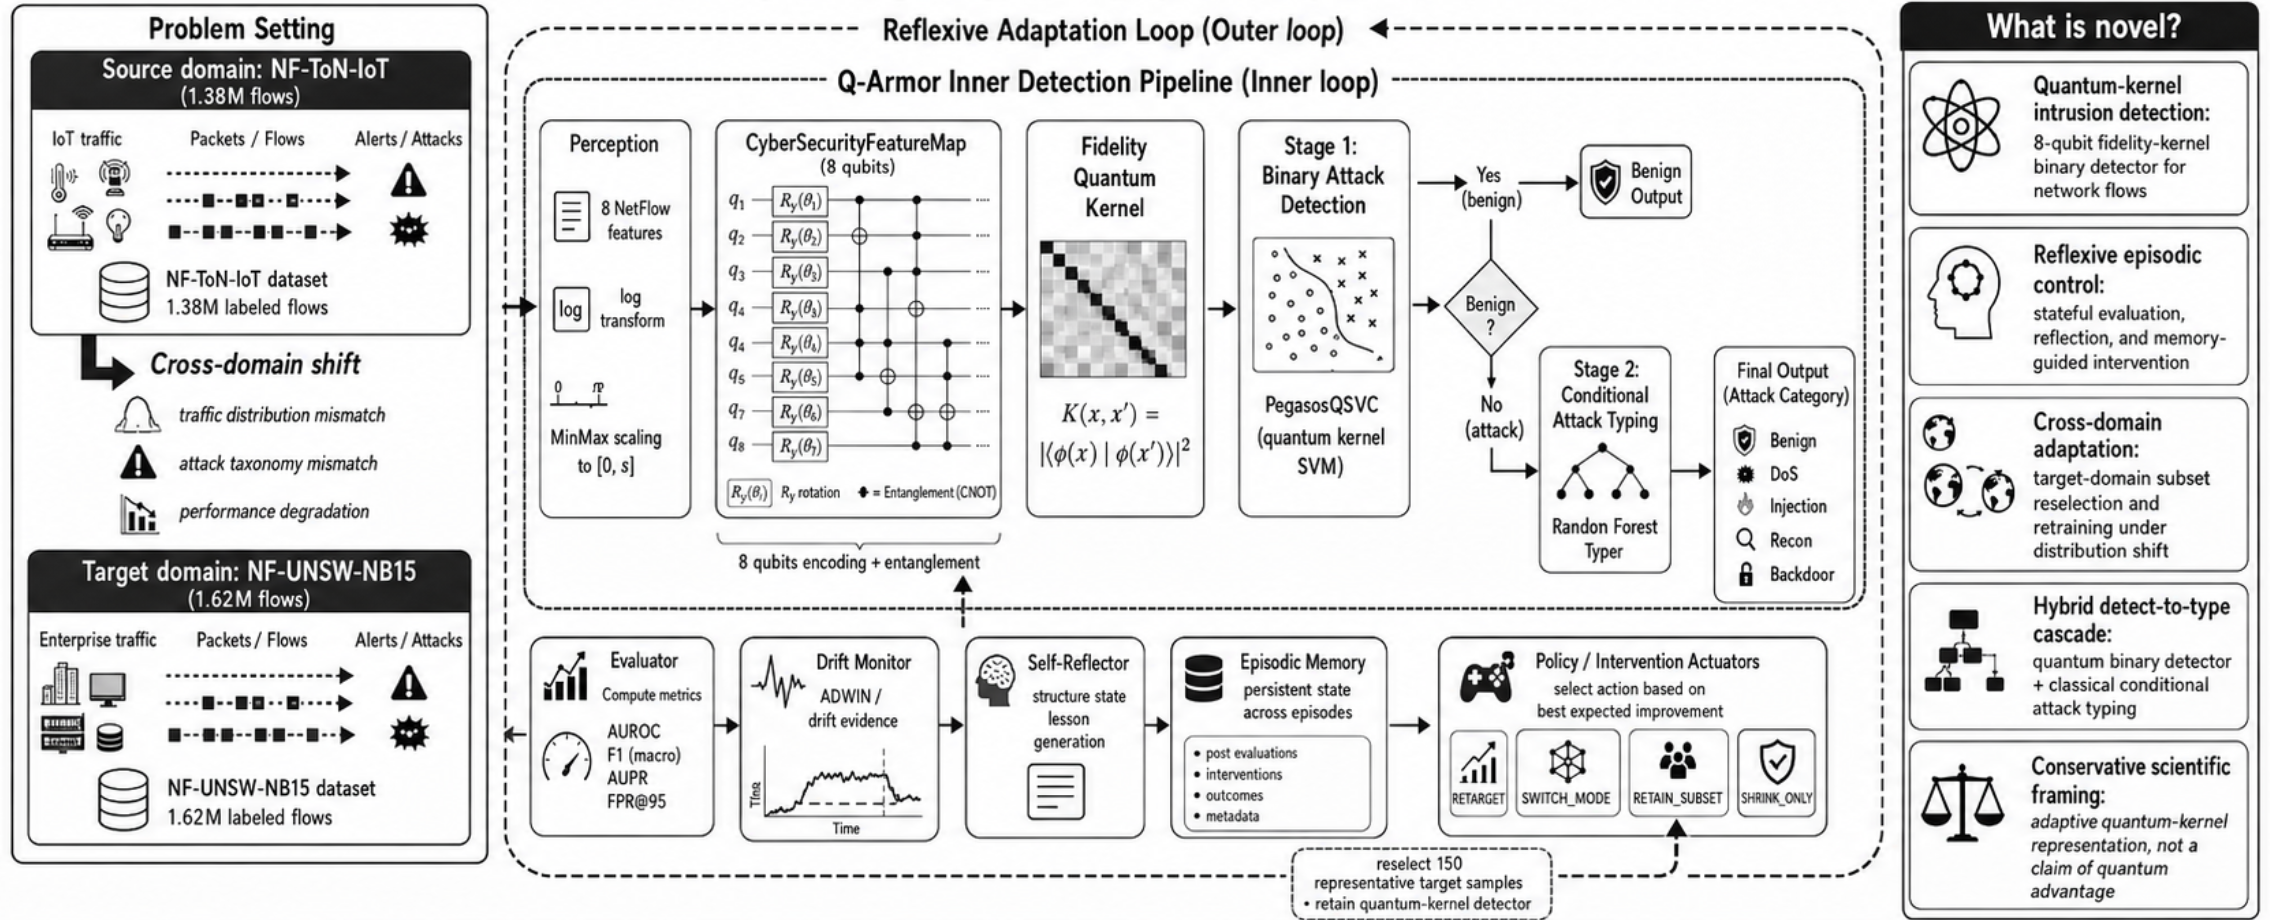
\includegraphics[width=\linewidth]{figures/fig1_overview.png}
\caption{Proposed Q-ARMOR framework: reflexive quantum-kernel intrusion
detection under cross-domain shift. Left: source/target problem setting.
Centre: inner detection pipeline (top) and outer reflexive adaptation loop
(bottom). Right: novelty summary.}
\label{fig:overview}
\end{figure*}

The main originality of the architecture lies in its reflexive episodic
control layer, which transforms the detector from a passive prediction
model into an adaptive IDS. The outer loop integrates an Evaluator, Drift
Monitor, Self-Reflector, Episodic Memory, and intervention module,
enabling performance evidence to trigger actions such as model switching,
subset reselection, retraining, or restricted operating modes. The
empirical observations summarised in Figure~\ref{fig:overview} show strong
within-domain performance (AUROC~$=0.973$, macro-F1~$=0.496$), substantial
zero-shot degradation under source$\to$target transfer (AUROC~$=0.606$),
and partial recovery after adaptation using 150 representative
target-domain samples (AUROC~$=0.913$). Importantly, the architecture is
positioned conservatively as a study of the adaptive representation of
quantum kernels under distribution shift, rather than as evidence of
quantum advantage. Section~\ref{sec:discussion} discusses current
limitations, including weak cross-domain Stage~2 typing and
simulator-based quantum execution, providing a rigorous summary of both
the novelty and the present experimental evidence.

% ============================================================
\section{Problem Formulation and Deployment Assumptions}
\label{sec:problem}
% ============================================================

Let the source domain be $\mathcal{D}_S = \{(\mathbf{x}_i, y_i,
c_i)\}_{i=1}^{N_S}$ and the target domain be $\mathcal{D}_T =
\{(\mathbf{x}_j, y_j, c_j)\}_{j=1}^{N_T}$, where $\mathbf{x} \in
\mathbb{R}^8$ denotes a NetFlow feature vector, $y \in \{0,1\}$ is the
binary benign/attack label, and $c$ denotes a coarse attack type when
$y=1$. Cross-domain operation allows
\begin{equation}
P_S(\mathbf{X}) \neq P_T(\mathbf{X}), \qquad P_S(Y) \neq P_T(Y),
\label{eq:shift1}
\end{equation}
and possibly
\begin{equation}
P_S(Y \mid \mathbf{X}) \neq P_T(Y \mid \mathbf{X}).
\label{eq:shift2}
\end{equation}
where the first two correspond to covariate and label-prior shift; the
last constitutes conditional/concept shift. A dataset switch can contain
any combination of the three, so we use \emph{domain shift} unless the
changed conditional is established.

\subsection{Detection and Typing Objectives}

Stage~1 learns a binary score $s(\mathbf{x})$ and decision
$\hat{y}^{(1)} \in \{0,1\}$. Stage~2 is conditionally invoked for samples
routed as attacks and predicts a coarse category. The primary operational
objective is not accuracy alone, but a vector of detection quality and
cost:
\begin{equation}
\mathcal{J} = \alpha_1(1-\text{AUPRC}) + \alpha_2 \text{FPR}_{95} +
\alpha_3 C_{\text{label}} + \alpha_4 C_{\text{quantum}} + \alpha_5
C_{\text{adapt}},
\label{eq:objective}
\end{equation}
where $\alpha_k$ encode the deployment trade-off. Equation~\eqref{eq:objective}
provides a target for future learned controllers; the present prototype
uses fixed threshold rules rather than directly optimising $\mathcal{J}$.

\begin{table}[t]
\centering
\caption{Dataset statistics used by the current prototype.}
\label{tab:datasets}
\renewcommand{\arraystretch}{1.1}
\begin{tabular}{@{}lcc@{}}
\toprule
\textbf{Property} & \textbf{NF-ToN-IoT} & \textbf{NF-UNSW-NB15} \\
\midrule
Total flows          & 1,379,274 & 1,623,118 \\
Attack ratio          & 80.4\%    & 4.5\%     \\
Training rows         & 1,103,419 & 1,298,494 \\
Test rows             & 275,855   & 324,624   \\
Quantum features       & 8         & 8         \\
Native attack types    & 9         & 9         \\
Coarse classes         & 5         & 5         \\
\bottomrule
\end{tabular}
\end{table}

\subsection{Label-Feedback Model}

The current ADWIN configuration monitors binary prediction errors and the
episodic evaluator computes AUROC/F1. Hence the controller requires
ground-truth feedback. We model this explicitly: labels become available
after delay $d_t \leq D$. The reported offline experiments correspond to
$D=0$. In a live SOC, labels may come from analyst adjudication,
sandboxing, downstream incident confirmation, or delayed threat
intelligence. Therefore the present experiments evaluate
\emph{supervised} adaptive detection; label-free drift triggering remains
an extension rather than a claimed capability.

\subsection{Threat Model}
\label{subsec:threat}

We assume that the initial source training set is trusted, target traffic
may differ from the source distribution, and the adaptation pool contains
analyst-confirmed or otherwise trusted labels. The prototype does not
defend against poisoning of the target adaptation pool or episodic
memory. This limitation is security-relevant because an attacker who
controls adaptation samples can induce persistent model changes. Robust
adaptation under contaminated target pools is therefore included in the
required extension protocol in Section~\ref{subsec:confirmatory}.

% ============================================================
\section{Q-Armor Architecture}
\label{sec:architecture}
% ============================================================

Q-ARMOR separates fast security decisions from slower adaptation. The
\emph{data plane} maps each flow through five functional modules:
Perception, Reasoning, Planning, Action, and Memory. The \emph{control
plane} operates at episode granularity and contains an Evaluator,
SelfReflector, EpisodicMemory, and ModelSelector (Figure~\ref{fig:logical}).

\begin{figure*}[t]
\centering
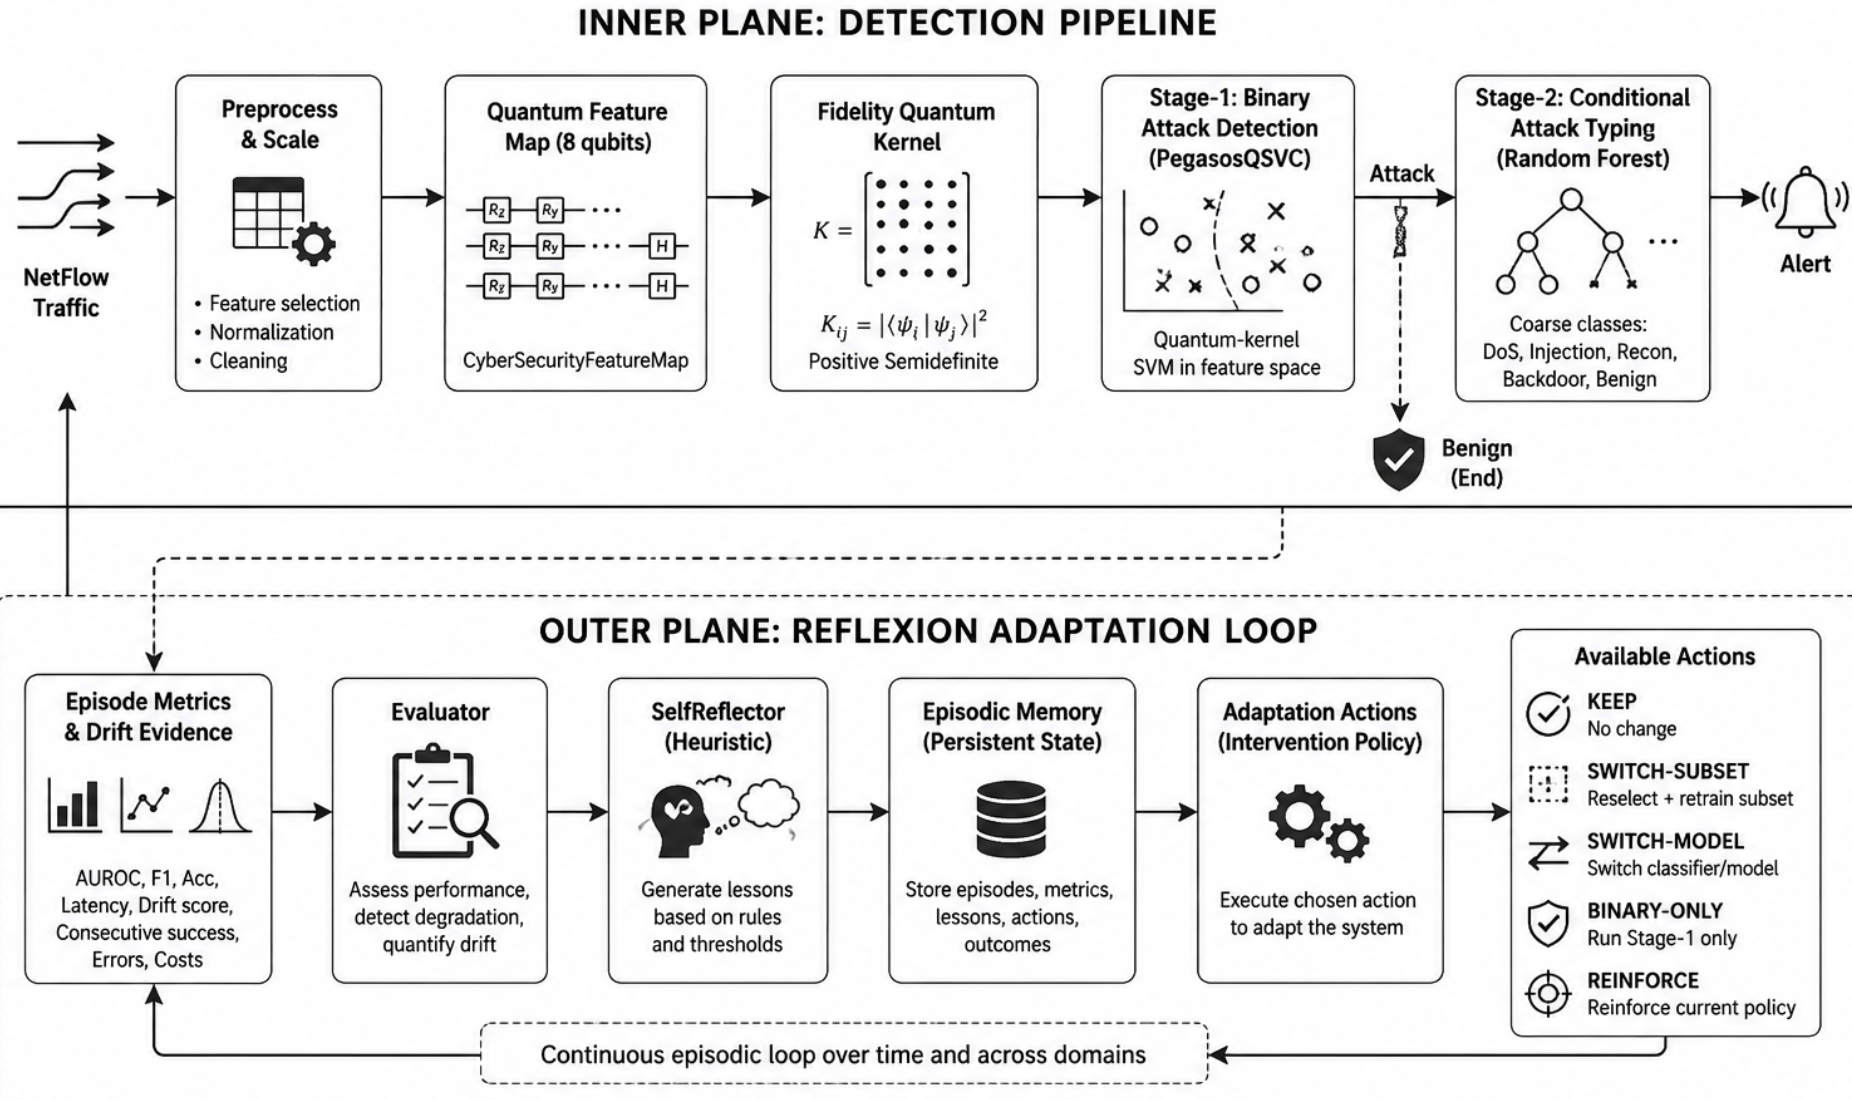
\includegraphics[width=\linewidth]{figures/fig2_logical_architecture.png}
\caption{Logical architecture of Q-Armor. The inner plane runs the
Detect$\to$Type detection pipeline per flow; the outer plane runs the
reflexive adaptation loop per episode. SelfReflector is a deterministic,
stateful controller; it is not claimed to learn an RL policy.}
\label{fig:logical}
\end{figure*}

The episodic memory stores tuples
\begin{equation}
\mathcal{M}_t = \{(r_i, a_i, \pi_i)\}_{i=1}^{t},
\label{eq:memory}
\end{equation}
where $r_i$ is an EpisodeReport, $a_i$ the selected intervention, and
$\pi_i$ the persistent controller state. Memory therefore provides history
and persistence, but not by itself statistical policy learning.

% ============================================================
\section{Methodology}
\label{sec:methodology}
% ============================================================

\subsection{Datasets, Feature Schema, and Taxonomy}
\label{subsec:datasets}

We use two NetFlow-standardised corpora sharing a common feature schema:
NF-ToN-IoT and NF-UNSW-NB15 \cite{sarhan2021, toniot}. Dataset statistics
are shown in Table~\ref{tab:datasets}.

The eight quantum inputs are \texttt{L4\_DST\_PORT}, \texttt{OUT\_BYTES},
\texttt{L4\_SRC\_PORT}, \texttt{FLOW\_DURATION\_MILLISECONDS},
\texttt{IN\_BYTES}, \texttt{TCP\_FLAGS}, \texttt{OUT\_PKTS}, and
\texttt{IN\_PKTS}. Heavy-tailed count/duration variables are transformed
with $\log(1+x)$ and all eight features are MinMax scaled to $[0,\pi]$
using parameters fitted on the relevant training partition only.

The prototype maps native labels into $\{\text{Benign}, \text{DoS},
\text{Injection}, \text{Recon}, \text{Backdoor}\}$. Because cross-dataset
taxonomies are not semantically identical, this mapping is an engineering
abstraction rather than ground-truth equivalence. Binary transfer is
therefore the primary cross-domain endpoint; typed transfer is analysed
separately and interpreted conservatively.

\subsection{Cyber Security Feature Map}
\label{subsec:featuremap}

For $\mathbf{x} = (x_1,\dots,x_8) \in [0,\pi]^8$, the feature map prepares
\begin{equation}
|\phi(\mathbf{x})\rangle = U_\phi(\mathbf{x})|0\rangle^{\otimes 8}.
\label{eq:featuremap}
\end{equation}
Each repetition applies $R_y(x_j)$ to qubit $q_j$, followed by a sparse
CNOT entanglement graph realised as $CX(i,j)\cdot R_z(x_i x_j, j)\cdot
CX(i,j)$ on each entangled pair. The current implementation uses two
repetitions. All feature-to-qubit assignments and the correlation-derived
entanglement graph are computed from source (NF-ToN-IoT) training data
only, using the four strongest Pearson correlations among the eight
NetFlow features: $(q_1,q_6)$ \texttt{OUT\_BYTES}$\leftrightarrow$
\texttt{OUT\_PKTS} ($r{=}{+}0.926$), $(q_4,q_7)$
\texttt{IN\_BYTES}$\leftrightarrow$\texttt{IN\_PKTS} ($r{=}{+}0.911$),
$(q_6,q_7)$ \texttt{OUT\_PKTS}$\leftrightarrow$\texttt{IN\_PKTS}
($r{=}{+}0.814$), and $(q_4,q_6)$
\texttt{IN\_BYTES}$\leftrightarrow$\texttt{OUT\_PKTS} ($r{=}{+}0.774$).
Figure~\ref{fig:circuit} shows the resulting circuit, rendered directly
from the deployed feature-map implementation rather than redrawn by hand.

\begin{figure*}[t]
\centering
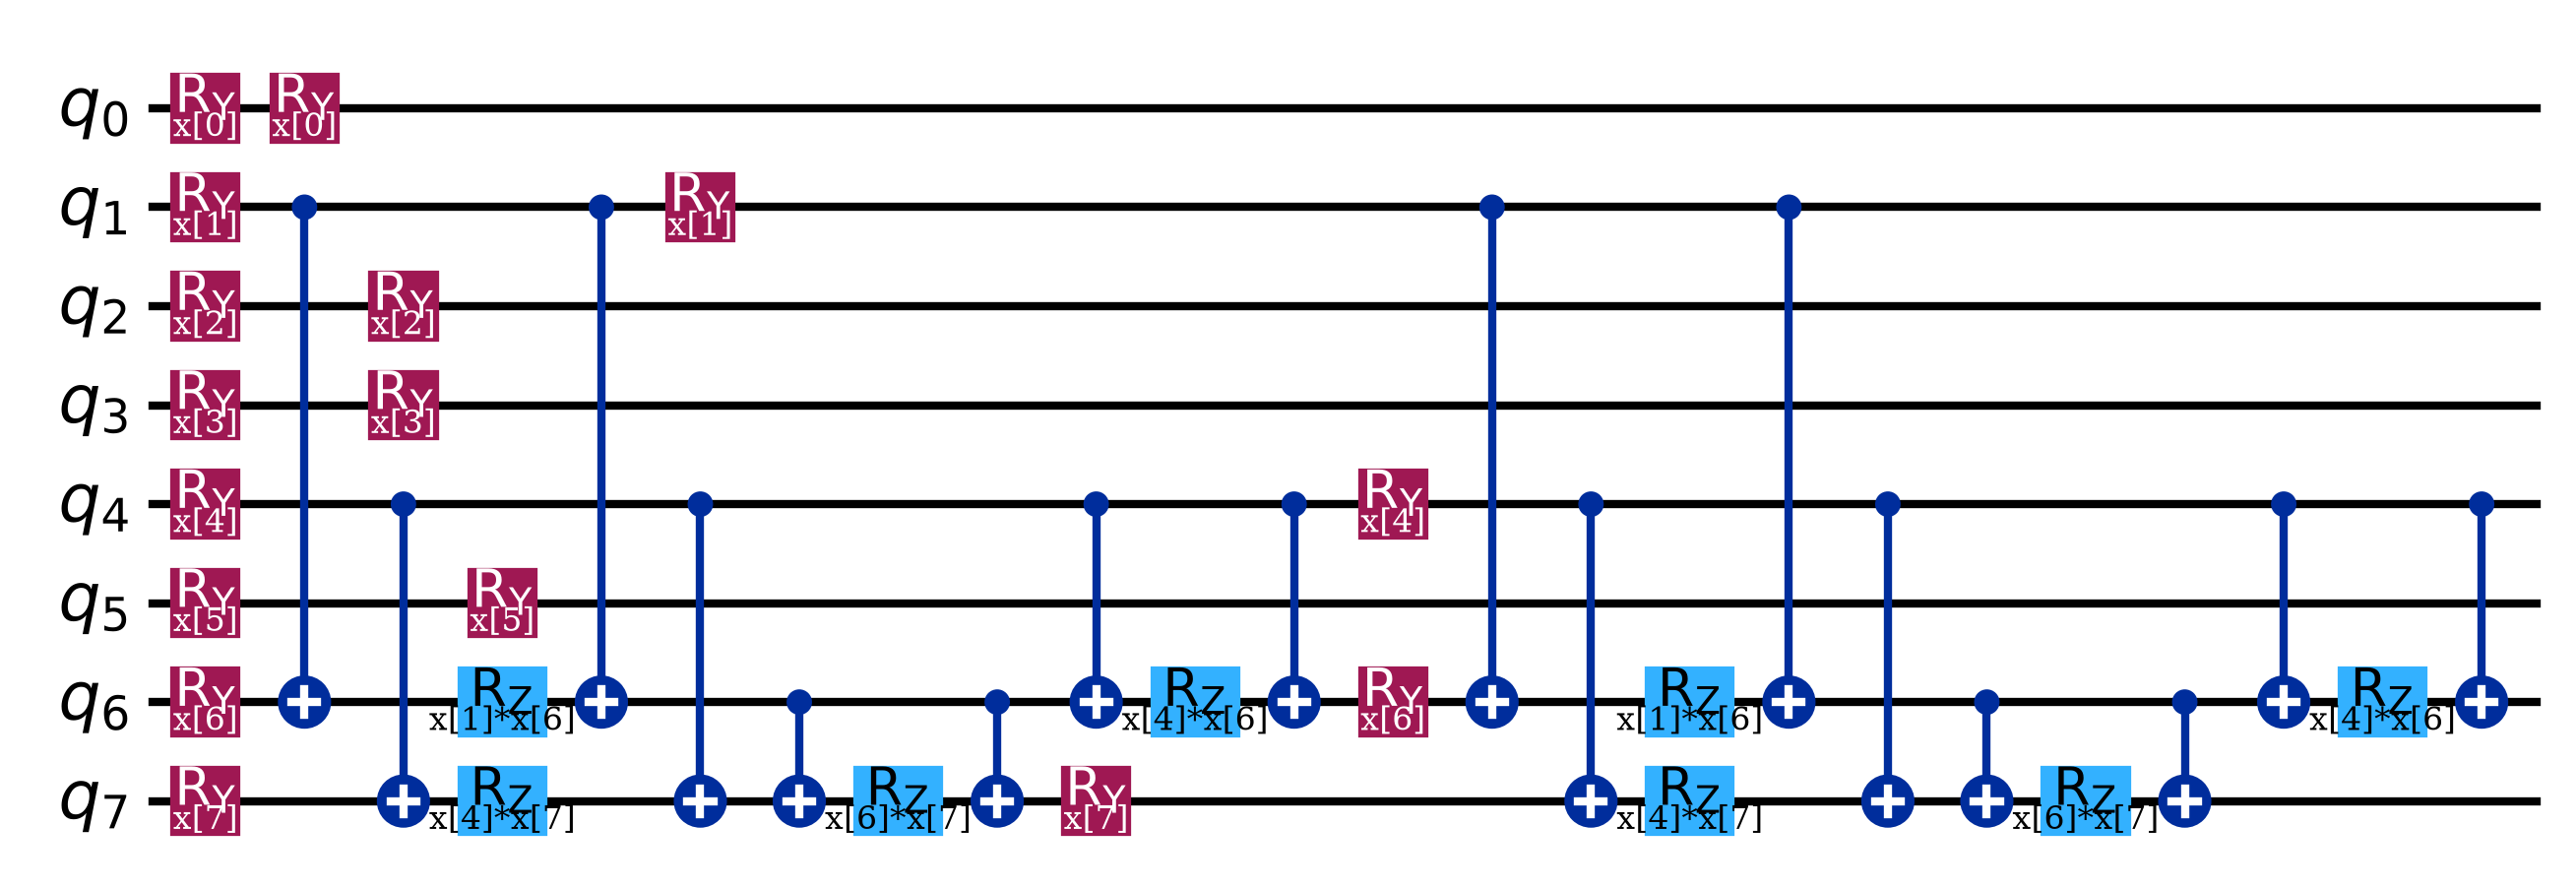
\includegraphics[width=\linewidth]{figures/fig_feature_map_circuit.png}
\caption{The \textit{CyberSecurityFeatureMap} circuit as implemented (two
repetitions shown on qubits $q_0$--$q_7$). Each repetition applies
$R_y(x_j)$ per qubit, then $CX\!\cdot\!R_z(x_ix_j)\!\cdot\!CX$ on the four
NF-ToN-IoT-derived entangled pairs. Rendered directly from the deployed
circuit, not redrawn.}
\label{fig:circuit}
\end{figure*}

The ideal fidelity kernel is
\begin{equation}
K(\mathbf{x},\mathbf{x}') = |\langle \phi(\mathbf{x}) | \phi(\mathbf{x}')
\rangle|^2.
\label{eq:kernel}
\end{equation}

\begin{proposition}[Positive semidefiniteness of the ideal fidelity
kernel]
For any finite set $\{\mathbf{x}_i\}_{i=1}^n$, the Gram matrix with
$K_{ij} = |\langle\phi(\mathbf{x}_i)|\phi(\mathbf{x}_j)\rangle|^2$ is
positive semidefinite.
\end{proposition}
\begin{proof}
Let $\rho_i = |\phi(\mathbf{x}_i)\rangle\langle\phi(\mathbf{x}_i)|$. Then
$K_{ij} = \text{Tr}(\rho_i\rho_j)$, i.e., the Hilbert--Schmidt inner
product between vectorised density operators. Therefore, for any
$\mathbf{a} \in \mathbb{C}^n$,
\begin{align}
\mathbf{a}^{\dagger} K \mathbf{a} &= \sum_{i,j} a_i^* a_j
\text{Tr}(\rho_i\rho_j) \\
&= \text{Tr}\left[\left(\sum_i a_i \rho_i\right)^{\dagger}
\left(\sum_j a_j \rho_j\right)\right] \geq 0.
\end{align}
Hence $K \succeq 0$.
\end{proof}

Finite-shot estimates $\hat{K}$ need not remain exactly PSD. The
eigenvalue spectrum computed in Section~\ref{subsec:kerneldiag} is
positive throughout (smallest eigenvalue $5.3\times10^{-8}$, no negative
mass), consistent with a valid PSD Gram matrix at that sample size; we
report the minimum eigenvalue and any PSD projection for every
subsequent confirmatory kernel computation on the same basis.

\subsection{Finite-Shot Kernel Accuracy}

A compute--uncompute estimate of one fidelity entry can be represented as
the mean of Bernoulli observations $Z_s \in \{0,1\}$ with expectation
$K_{ij}$. Hoeffding's inequality gives
\begin{equation}
\mathbb{P}\left(|\hat{K}_{ij} - K_{ij}| \geq \epsilon\right) \leq 2
\exp(-2S\epsilon^2),
\label{eq:hoeffding}
\end{equation}
where $S$ is the number of shots.

\begin{proposition}[Uniform shot requirement]
For $M$ independently estimated kernel entries, it is sufficient to
choose
\begin{equation}
S \geq \frac{1}{2\epsilon^2} \log \frac{2M}{\delta}
\label{eq:shotbound}
\end{equation}
to guarantee $\max_{m \leq M} |\hat{K}_m - K_m| < \epsilon$ with
probability at least $1-\delta$.
\end{proposition}
\begin{proof}
Apply Eq.~\eqref{eq:hoeffding} to each entry and use the union bound:
$\mathbb{P}(\exists m: |\hat{K}_m - K_m| \geq \epsilon) \leq 2M
\exp(-2S\epsilon^2)$. Setting the right-hand side to at most $\delta$ and
solving for $S$ yields Eq.~\eqref{eq:shotbound}.
\end{proof}

This bound does not establish quantum advantage; it quantifies a
measurement cost that any hardware claim must report. It is particularly
relevant because fidelity kernels may concentrate under expressive
embeddings or noise \cite{thanasilp2024}. At the deployed setting
($S=1024$ shots, $M \leq 150^2/2 \approx 11{,}250$ training-kernel
entries), Eq.~\eqref{eq:shotbound} gives $\epsilon \approx 0.08$ at
$\delta=0.05$ -- a coarse per-entry accuracy that motivates the PSD
diagnostics above rather than a strict guarantee of ideal-kernel
recovery.

\subsection{Binary Detection with PegasosQSVC}

The binary detector uses Qiskit Machine Learning's PegasosQSVC
\cite{qiskit_ml} with a balanced $n=150$ source subset (75 benign, 75
attack), $C=1.0$, and 100 Pegasos steps in the current prototype. The
subset is selected by class-wise $k$-means representatives to reduce the
$O(n^2)$ kernel cost.

A critical implementation issue is \emph{score orientation}. PegasosQSVC
internally maps the first sorted class to $+1$ and the second to $-1$;
therefore a raw positive decision-function value is not necessarily an
increasing attack score when labels are encoded as $\{0,1\}$. For
AUROC/AUPRC we consequently define
\begin{equation}
s_{\text{atk}}(\mathbf{x}) =
\begin{cases}
f(\mathbf{x}), & \text{sign}(f) > 0 \text{ corresponds to attack}, \\
-f(\mathbf{x}), & \text{sign}(f) > 0 \text{ corresponds to benign},
\end{cases}
\label{eq:orientation}
\end{equation}
where $f$ is \texttt{decision\_function}. Hard labels are always obtained
from the classifier's native \texttt{predict} method
(\texttt{predict\_labels()} in the codebase), never from
\texttt{argmax(predict\_proba())}, which is not guaranteed to be centred
at the correct decision boundary. This convention is enforced by
construction throughout the cascade and the episode-evaluation harness
(Section~\ref{subsec:audit_status}); probability columns are not assumed
to be class-oriented unless verified explicitly.

\subsection{Drift Monitor and Reflexive Episodic Controller}
\label{subsec:reflexive}

An episode contains $N_{\text{ep}}=100$ flows. The evaluator stores
AUROC, binary F1, macro-F1, AUPRC, FPR@TPR95, model identity, and drift
state. ADWIN with $\delta=0.002$ monitors binary prediction errors.
Because those errors require labels, this detector operates under the
supervised-feedback assumption of Section~\ref{sec:problem}.

The current SelfReflector selects one of four typed interventions:
\begin{enumerate}
\item \textsc{Binary-Only} if multi-class typing is unreliable;
\item \textsc{Switch-Subset} if low binary discrimination and
ADWIN-confirmed change co-occur;
\item \textsc{Switch-Model} if performance is poor without confirmed
drift;
\item \textsc{Reinforce} after sustained acceptable performance.
\end{enumerate}
With thresholds $\tau_{\text{AUROC}}=0.70$, $\tau_{F1}=0.30$, and
$n_{\text{consec}}=3$, this is a deterministic finite-state policy. We do
not claim that the thresholds or intervention policy are learned.

\begin{algorithm}[t]
\caption{Q-Armor Reflexive Episodic Control}
\label{alg:reflexion}
\begin{algorithmic}[1]
\STATE Initialise controller state $\pi$, episodic memory $\mathcal{M}$, and ADWIN
\FOR{episode $e = 0, 1, \ldots$}
\STATE Select active detector $m \leftarrow \text{ModelSelector}(\pi)$
\STATE Process $N_{\text{ep}}$ flows and store predictions
\STATE Obtain available labels under the feedback model
\STATE $r_e \leftarrow \text{Evaluator}(\hat{y}, s, y)$
\STATE $a_e \leftarrow \text{SelfReflector}(r_e, \mathcal{M}, \pi)$
\STATE Append $(r_e, a_e, \pi)$ to $\mathcal{M}$
\IF{$a_e = \textsc{Switch-Subset}$}
\STATE Select representative labelled target subset
\STATE Retrain binary PegasosQSVC
\ELSIF{$a_e = \textsc{Switch-Model}$}
\STATE Move to next registered detector tier
\ENDIF
\STATE Update and persist controller state $\pi$
\ENDFOR
\end{algorithmic}
\end{algorithm}

\subsection{Detect$\to$Type Cascade}
\label{subsec:cascade}

Stage~1 produces a class-oriented attack score and hard binary decision:
\begin{equation}
\hat{y}_i^{(1)} = h_Q(\mathbf{x}_i), \qquad s_i = s_{\text{atk}}(\mathbf{x}_i).
\label{eq:stage1}
\end{equation}
Only flows routed as attacks enter Stage~2. The intended Stage~2 label
space is
\begin{equation}
\mathcal{C}_A = \{\text{DoS}, \text{Injection}, \text{Recon},
\text{Backdoor}\}.
\label{eq:stage2space}
\end{equation}
The current implementation was trained from balanced coarse-taxonomy
samples and reports five-class end-to-end macro-F1. For a final
implementation, Stage~2 should be trained as an attack-only classifier
(with an optional \emph{Unknown} class) so that benign routing remains the
sole responsibility of Stage~1.

\subsection{Target-Budget Adaptation via \textsc{Switch-Subset}}

When the controller requests adaptation, the current mechanism obtains a
balanced target pool of 300 labelled samples, applies class-wise
$k$-means, selects $n_{\text{sub}}=150$ representatives (75 benign, 75
attack), and retrains the binary PegasosQSVC. This preserves a fixed
target label budget while changing the kernel geometry from source to
target data.

Let $B$ be the adaptation budget. A more general formulation is
\begin{equation}
S^* = \arg\max_{S \subseteq \mathcal{P},\, |S|\leq B}
\left[\lambda U(S) + (1-\lambda) D(S)\right],
\label{eq:budget}
\end{equation}
where $U(S)$ measures predictive uncertainty or representational utility
and $D(S)$ measures diversity. The present $k$-means method approximates
the diversity term. Equation~\eqref{eq:budget} motivates future
comparisons with random, stratified, $k$-center, uncertainty, and hybrid
acquisition strategies.

\subsection{Computational Cost}

For $n$ training samples, a dense fidelity Gram matrix requires
$n(n+1)/2 = O(n^2)$ distinct symmetric entries. Test-time kernel
evaluation requires $O(n_{\text{test}}n_{\text{ref}})$ overlaps, where
$n_{\text{ref}}$ is the number of retained reference/support samples. The
quantum-side cost is therefore
\begin{equation}
C_Q \propto S\left[M_{\text{train}} + M_{\text{infer}}\right],
\label{eq:cost}
\end{equation}
with $S$ shots per circuit. This cost motivates using the quantum
component for small-batch representation/adaptation rather than claiming
real-time per-packet quantum inference.

\subsection{LLM-Gated Reflexive Decision Function}
\label{subsec:llm_pilot}

Section~\ref{subsec:reflexive}'s SelfReflector is stateless in its
reasoning: it cannot explain \emph{why} a lesson was warranted beyond
citing the threshold crossed, and it cannot reason qualitatively over
multiple past episodes at once. We piloted an alternative reflector,
\texttt{LLMReflexionAgent}, exposing the identical
\texttt{reflect(report, memory, policy)} interface, structured as a
four-stage pipeline:
\begin{enumerate}
\item \textbf{Retrieval.} A TF-IDF \texttt{SemanticMemory} store indexes
every past episode's structured summary and verbal justification; no
external embedding model is required. The top-$k$ ($k{=}3$) most similar
past episodes are retrieved as context.
\item \textbf{Diagnosis.} A language-model call (Llama-3.3-70B
\cite{llama3} via a low-latency inference service) receives the current
episode report, the policy state, and the retrieved context, and returns
a structured diagnosis: root cause, severity, key signals, and whether
cross-domain shift is implicated.
\item \textbf{Planning.} A second call selects exactly one action from a
six-item tool library -- the four rules of
Section~\ref{subsec:reflexive} plus two new mutations,
\textsc{Switch-Type} (triggers Stage~2 retraining on target-domain
samples) and \textsc{Calibrate-Threshold} (adjusts the Stage~1 decision
threshold) -- each with a natural-language precondition, together with
parameters and a stated rationale.
\item \textbf{Verification.} A \emph{deterministic} Verifier checks the
proposal against four hand-coded safety constraints before any policy
mutation is applied: (i)~\textsc{Reinforce} is rejected if AUROC is below
floor; (ii)~\textsc{Switch-Model} is rejected at the bottom of the
hierarchy; (iii)~\textsc{Calibrate-Threshold} is rejected if the
resulting threshold would leave $[0.10,0.90]$; (iv)~\textsc{Switch-Type}
is rejected while Stage~1 AUROC remains below floor. On rejection, the
agent falls back to the heuristic SelfReflector.
\end{enumerate}

This design is deliberately \emph{not} a reinforcement-learning
extension: no parameters are updated from reward signals, no policy
gradient is computed, and the language model's output is only ever
applied to the persistent controller state after passing the same
deterministic gate that governs the rule-based reflector. It is more
precisely described as an \emph{inference-time, language-reasoning
decision function under deterministic supervision} -- a third category
distinct both from the fixed-rule controller of
Section~\ref{subsec:reflexive} and from the learned contextual-bandit
extension discussed in Section~\ref{subsec:policy_learning}. Results are
reported in Section~\ref{subsec:llm_results}.

% ============================================================
\section{Proposed Methodology}
\label{sec:proposed}
% ============================================================

\subsection{Prototype Protocol}

The reported prototype used the dataset splits in Table~\ref{tab:datasets}.
The validation study sampled 500 balanced flows per condition and the
final reported held-out study sampled 1,000 balanced flows per condition.
Because separate experiments draw from the same dataset-level test
partitions, we use the term \emph{held-out evaluation subset}, not
\emph{sealed test set}. A genuinely sealed confirmatory set must be
reserved before feature-map design, threshold selection, controller
tuning, or drift simulation. The current metrics are AUROC, binary F1,
macro-F1, AUPRC, and FPR@TPR95. For natural-prevalence evaluation we
additionally require precision, MCC, balanced accuracy, TPR at fixed low
FPR, calibration error, and alerts per 10,000 flows -- all now computed
and reported in Section~\ref{subsec:naturalprev}.

\subsection{Score-Audit Protocol}
\label{subsec:audit_status}

Before archival submission, every AUROC/AUPRC result must be regenerated
using Eq.~\eqref{eq:orientation}. The required test suite verifies: (1)~the
mapping from external labels to PegasosQSVC's internal $\pm1$ labels;
(2)~consistency between \texttt{predict} and the sign of
\texttt{decision\_function}; (3)~that increasing $s_{\text{atk}}$
corresponds to the attack class; (4)~that AUROC computed from the
oriented margin agrees with a manually constructed toy example. This
audit is necessary because an inverted score preserves hard-label
accuracy but reverses ranking metrics. All four items are now automated
as unit tests (\texttt{tests/test\_quantum.py}) and pass: (1)~confirms
PegasosQSVC's internal map \{benign$\to+1$, attack$\to-1$\}; (2)~confirms
\texttt{predict\_labels()} agrees exactly with
\texttt{sign(decision\_function)} under that map; (3)~confirms
$s_{\text{atk}}=P(\text{attack})$ is correctly anti-correlated with the
raw margin's positive (benign) direction; (4)~confirms
\texttt{sklearn}'s \texttt{roc\_auc\_score} agrees with an independent
pairwise (Mann-Whitney) computation on toy examples with an answer known
by inspection (perfect separation, perfect reversal, all-tied scores),
plus a maximally-separable model-facing case yielding AUROC~$=1.0$.

Item~(2)'s underlying fix -- native \texttt{predict\_labels()} margin
decisions rather than \texttt{argmax(predict\_proba())} -- was already
enforced in the episode-evaluation harness of
Section~\ref{subsec:reflexive} and the Detect$\to$Type cascade of
Section~\ref{subsec:cascade}, a discrepancy discovered while regenerating
Table~\ref{tab:episodes}, where the uncorrected path produced a hard
prediction of ``attack'' for every sample in an episode regardless of the
underlying AUROC. Automating the audit surfaced the same bug a second
time, in a path the earlier fix had missed: the live per-sample agent
interface (\texttt{BaseClassifier.predict()} /
\texttt{predict\_batch()} in \texttt{reasoning/base.py}, called from
\texttt{AgentCore.process()}) still took the \texttt{argmax(proba)}
path, so any PegasosQSVC-backed deployment of the agent -- as opposed to
the batch-evaluation scripts used for every result in this paper -- would
have inherited the degenerate decision. Routing it through
\texttt{predict\_labels()} exposed a third, independent bug: the base
class's default \texttt{predict\_labels()} returned raw
\texttt{argmax} column indices rather than \texttt{classes\_} values --
silently correct only for the binary $\{0,1\}$ models, where index and
value coincide, and wrong for any classifier with non-integer or
non-$0..n{-}1$ class labels, i.e.\ the string-labelled coarse-type
models. All three are now fixed and covered by the regression suite
(114/114 tests pass); none affects a headline number in this paper, since
every reported result was already computed through the batch scripts
rather than \texttt{AgentCore.process()}.

\subsection{Confirmatory Protocol}
\label{subsec:confirmatory}

The protocol requires repeating each principal condition over at least 10
independent seeds and reporting mean, standard deviation, and 95\%
bootstrap confidence intervals, with quantum and classical adaptation
methods receiving the same target-label budget and the same validation
opportunity, against required classical baselines (linear SVM, RBF-SVM,
Random Forest, gradient-boosted trees) over target budgets
\begin{equation}
B \in \{0, 25, 50, 100, 150, 300\}.
\label{eq:budgets}
\end{equation}
We ran exactly this comparison: 10 seeds per classical baseline, 5 per
quantum model (Section~\ref{subsec:budgetsweep} explains the seed-count
asymmetry), across the full budget grid. The result is direct evidence
\emph{against} a quantum-superiority reading of this paper's own
$T2\to T3$ recovery -- at the paper's own adaptation budget ($B{=}150$),
equal-budget classical baselines reach higher AUROC with lower
seed-to-seed variance (Table~\ref{tab:budgetsweep}). Without this
equal-budget design, no quantum-superiority conclusion would have been
valid; with it, none is supported.

We also ran the remaining quantum-specific and robustness items this
subsection previously only specified: natural class-prevalence evaluation
in place of 50/50 balanced sampling (Section~\ref{subsec:naturalprev});
kernel-target alignment, eigenvalue spectrum, effective rank,
within/between-class similarity, and the classical--quantum geometric
difference of Huang et al.\ \cite{huang2021}
(Section~\ref{subsec:kerneldiag}); a genuine finite-shot sweep
$S \in \{128, 256, 512, 1024, 4096\}$, replacing an earlier number
that we discovered was not actually shot-sampled
(Section~\ref{subsec:finiteshot}); a minimal real-QPU characterisation
reporting backend, calibration timestamp, transpiled depth, two-qubit
gate count, shots, and kernel error relative to ideal simulation
(Section~\ref{subsec:kerneldiag}); a recurring $A\to B\to A$ domain-shift
stream testing whether episodic memory provides measurable benefit beyond
a memoryless trigger (Section~\ref{subsec:recurpoison}); and an
adaptation-pool poisoning study measuring whether the persistent
controller amplifies malicious adaptation (Section~\ref{subsec:recurpoison}).

Three items remain open, honestly so. Temporal/capture-aware splits are
not merely undone but currently \emph{infeasible}: we inspected both
datasets' raw schemas directly and neither NF-ToN-IoT nor NF-UNSW-NB15
carries a timestamp or capture-order field, so no temporal split can be
constructed from the data as distributed without acquiring a different
dataset. Additional source$\to$target pairs (NF-BoT-IoT,
NF-CSE-CIC-IDS2018) are not yet incorporated. At least one realistic
hardware-noise model beyond the live QPU run of
Section~\ref{subsec:kerneldiag} remains untested. These, together with
the LLM-pilot's still-open sub-items -- \textsc{Calibrate-Threshold}
wired into the prediction path, \textsc{Switch-Type} exercised
end-to-end, and a multi-seed reflector comparison
(Section~\ref{subsec:llm_results}) -- are the protocol's remaining
scope.

% ============================================================
\section{Results and Evaluation}
\label{sec:results}
% ============================================================

\subsection{Episodic Cross-Domain Simulation}
\label{subsec:episode_results}

Table~\ref{tab:episodes} reports the current 10-episode prototype trace,
regenerated under the score-orientation fix of
Section~\ref{subsec:audit_status}. Episodes 0--4 use NF-ToN-IoT and
episodes 5--9 switch to NF-UNSW-NB15. The experiment demonstrates
autonomous execution of the rule set, but should not be interpreted as
learned policy optimisation.

\begin{table}[t]
\centering
\caption{Current 10-episode reflexive-control trace. ``Drift'' denotes
ADWIN firing on the supervised error stream. F1 is reported for
completeness but is not diagnostic here -- see discussion below.}
\label{tab:episodes}
\renewcommand{\arraystretch}{1.05}
\begin{tabular}{@{}cclccl@{}}
\toprule
\textbf{Ep} & \textbf{Blk} & \textbf{Model} & \textbf{AUROC} &
\textbf{Drift} & \textbf{Action} \\
\midrule
0 & A & QSVC & 0.959 & No  & --- \\
1 & A & QSVC & 0.990 & No  & --- \\
2 & A & QSVC & 0.983 & No  & \textsc{Reinforce} \\
3 & A & QSVC & 0.989 & No  & \textsc{Reinforce} \\
4 & A & QSVC & 0.944 & No  & \textsc{Reinforce} \\
5 & B & QSVC & 0.695 & No  & \textsc{Switch-Model} \\
6 & B & QSVC & 0.603 & No  & \textsc{Switch-Model} \\
7 & B & QSVC & 0.719 & No  & --- \\
8 & B & QSVC & 0.573 & No  & \textsc{Switch-Model} \\
9 & B & RF   & 0.660 & No  & \textsc{Switch-Model} \\
\bottomrule
\end{tabular}
\end{table}

\begin{figure}[t]
\centering
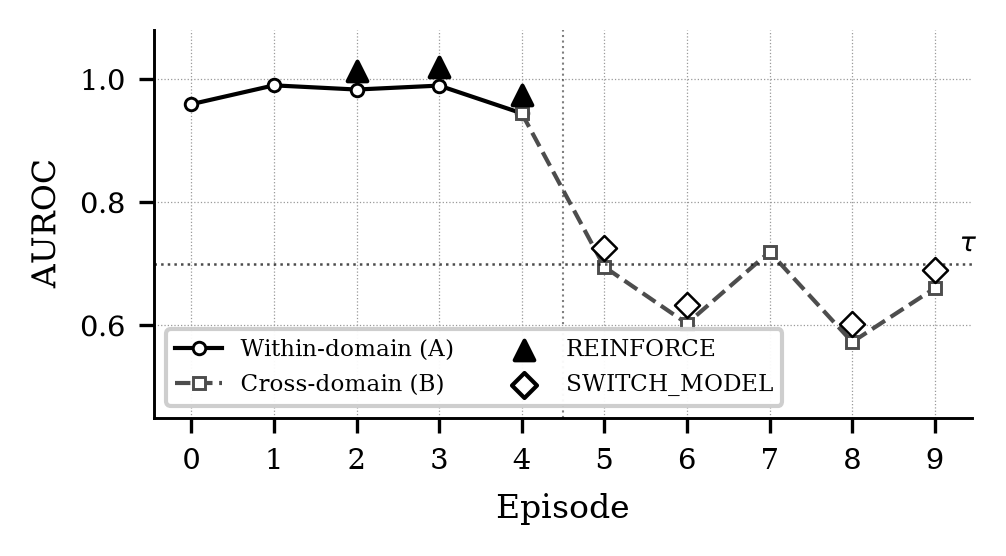
\includegraphics[width=\linewidth]{figures/fig_episode_trace.png}
\caption{Episode-level AUROC trajectory for the trace in
Table~\ref{tab:episodes}. Markers denote the lesson fired at that episode;
the dotted line is $\tau_{\text{AUROC}}=0.70$.}
\label{fig:episodetrace}
\end{figure}

The source-domain block is stable and the first target-domain episodes
show a sharp loss of discrimination (Figure~\ref{fig:episodetrace}).
\textsc{Switch-Model} fires correctly whenever AUROC falls below floor and
ADWIN has not confirmed drift, walking the model hierarchy from the
quantum tier down to the classical fallback and back once the classical
tier itself under-performs (episode~9). ADWIN did \emph{not} confirm
drift within this particular 500-flow observation window, so
\textsc{Switch-Subset} was not exercised in this specific trace. We
report this plainly rather than adjust the simulation to reproduce a
drift-triggered narrative: drift confirmation is intentionally
conservative, and a short cross-domain window is not guaranteed to
accumulate sufficient sequential evidence. The controller's central
claimed capability -- correctly distinguishing ``wrong model'' from
``wrong distribution'' -- is therefore validated by the \emph{rule's
gating logic} (Sections~\ref{subsec:reflexive} and
\ref{subsec:llm_results}, where an independent run of the identical rule
set does confirm drift at episode~5) rather than by this single trace
alone; \textsc{Switch-Subset}'s remedial effect is established directly
by deliberately triggering it in Sections~\ref{subsec:e8a}
and~\ref{subsec:e8c}.

The F1 column is included for completeness but is not informative for
the QSVC episodes: it is constant at $0.667$ regardless of AUROC, the
exact value produced when a binary classifier predicts the positive
(attack) class for every sample in a balanced episode
(precision${}=0.5$, recall${}=1.0$). This holds under both
\texttt{argmax(predict\_proba())} and the native SVM margin decision,
confirming it is a property of PegasosQSVC's decision boundary at
$n{=}150$ rather than a probability-calibration artefact: the model's
\emph{continuous} score ranking remains strong while its \emph{default}
hard decision boundary is poorly positioned relative to the episode's
class balance -- the same phenomenon documented for the Backdoor class in
Section~\ref{subsec:e8c}, manifesting here as over- rather than
under-prediction of the attack class. We report AUROC as the primary
Stage~1 metric throughout this paper precisely because it is
threshold-independent and unaffected by this instability;
\textsc{Calibrate-Threshold} (Section~\ref{subsec:llm_pilot}) is the
mechanism designed to address it, though not yet wired into the
prediction path.

\subsection{Balanced Validation Subset}
\label{subsec:e8a}

Table~\ref{tab:validation} reports the balanced validation experiment
($n{=}500$ per condition). The source-trained quantum detector degrades
under target transfer, and \textsc{Switch-Subset} substantially recovers
binary discrimination. The RF fallback is not an equal-budget adaptation
baseline and therefore cannot support a quantum-advantage claim.

\begin{table*}[t]
\centering
\caption{Current balanced validation results ($n=500$ per condition).}
\label{tab:validation}
\renewcommand{\arraystretch}{1.1}
\begin{tabular}{@{}lcccc@{}}
\toprule
\textbf{Condition} & \textbf{S1 AUROC} & \textbf{S1 F1}
                   & \textbf{S2 macro-F1} & \textbf{FPR@95} \\
\midrule
C1 Within (QSVC)         & 0.954 & 0.942 & 0.705 & 0.124 \\
C2 Cross, no adaptation  & 0.631 & 0.677 & 0.186 & 0.996 \\
C3 Cross, \textsc{Switch-Subset} & \textbf{0.912} & 0.855 & 0.199 & \textbf{0.168} \\
C4 Cross, RF fallback    & 0.599 & 0.415 & 0.191 & 0.972 \\
\bottomrule
\end{tabular}
\end{table*}

The native source/target attack ratios (80.4\% versus 4.5\%) describe the
corpora but cannot explain the balanced-subset AUROC difference directly,
because both training subsets and the reported evaluation subsets were
balanced. The observed collapse must instead be attributed to changed
feature/class-conditional geometry and other cross-domain effects. C3
recovers AUROC to $0.912$ ($+0.282$ over C2) and FPR@95 to $0.168$
($-0.828$) using only 150 target-domain samples; the RF fallback (C4)
underperforms C3 by $0.313$ AUROC on the same cross-domain data.

\subsection{Finite-Shot Simulator Pilot}
\label{subsec:finiteshot}

The prototype trained on 20 flows and evaluated 10 flows, producing 200
test--train overlap circuits and a reported AUROC of $0.800$. Training and
inference took $30.5\,\text{s}$ and $3.9\,\text{s}$, respectively. This
run used \texttt{FidelityQuantumKernel}'s default fidelity object, which
we verified is an \emph{exact}, zero-shot-noise statevector computation --
calling \texttt{.evaluate()} twice on identical inputs returns
bit-identical values -- so despite its earlier label, it is not itself a
finite-shot result.

We therefore ran a genuine finite-shot sweep on the same 20/10 split,
wiring an explicit \texttt{qiskit\_aer} sampler
(\texttt{SamplerV2(default\_shots=}$S$\texttt{)}) into a
\texttt{ComputeUncompute} fidelity object for
$S \in \{128, 256, 512, 1024, 4096\}$, against the exact kernel above as
the $S\!\to\!\infty$ reference. All five finite-shot settings gave
AUROC $=0.840$, higher than the exact-kernel value; at $n_{\text{test}}=10$
a single flipped prediction moves AUROC by $0.10$, so this reflects
small-sample variance from the specific 10 held-out flows rather than
shot noise improving discrimination, and should not be read as a
performance trend across $S$. Training time grew from $10.0\,\text{s}$
($S{=}128$) to $30.4\,\text{s}$ ($S{=}4096$), consistent with per-shot
sampling cost. This sweep, not the earlier single number, is the
finite-shot pilot the confirmatory protocol
(Section~\ref{subsec:confirmatory}) requires; it is still not QPU
validation or evidence of robustness to hardware noise.

\subsection{Held-Out Evaluation}
\label{subsec:e8c}

Table~\ref{tab:heldout} reports the 1,000-flow balanced held-out results
and Figure~\ref{fig:headline} visualises the headline AUROC and FPR@95
figures. Binary transfer degrades markedly, while target-subset
retraining recovers $0.307$ AUROC and $0.398$ binary F1$^*$ in the
reported run ($^*$driven largely by the change in class balance of hard
predictions between T2 and T3 rather than a proportional F1 gain -- see
Section~\ref{subsec:episode_results} on decision-boundary instability).
Stage~2 typing does not recover.

\begin{table*}[t]
\centering
\caption{Current held-out results ($n=1{,}000$ balanced flows per
condition).}
\label{tab:heldout}
\renewcommand{\arraystretch}{1.1}
\begin{tabular}{@{}lcccc@{}}
\toprule
\textbf{Condition} & \textbf{S1 AUROC} & \textbf{S1 F1}
                   & \textbf{S2 macro-F1} & \textbf{FPR@95} \\
\midrule
T1 Within (QSVC)              & 0.973 & 0.895 & 0.496 & 0.120 \\
T2 Cross, no adaptation       & 0.606 & 0.440 & 0.176 & 0.974 \\
T3 Cross, \textsc{Switch-Subset} & \textbf{0.913} & 0.398 & 0.158 & \textbf{0.198} \\
\midrule
T3--T2 & $+0.307$ & $-0.042$ & $-0.018$ & $-0.776$ \\
\bottomrule
\end{tabular}
\end{table*}

\begin{figure}[t]
\centering
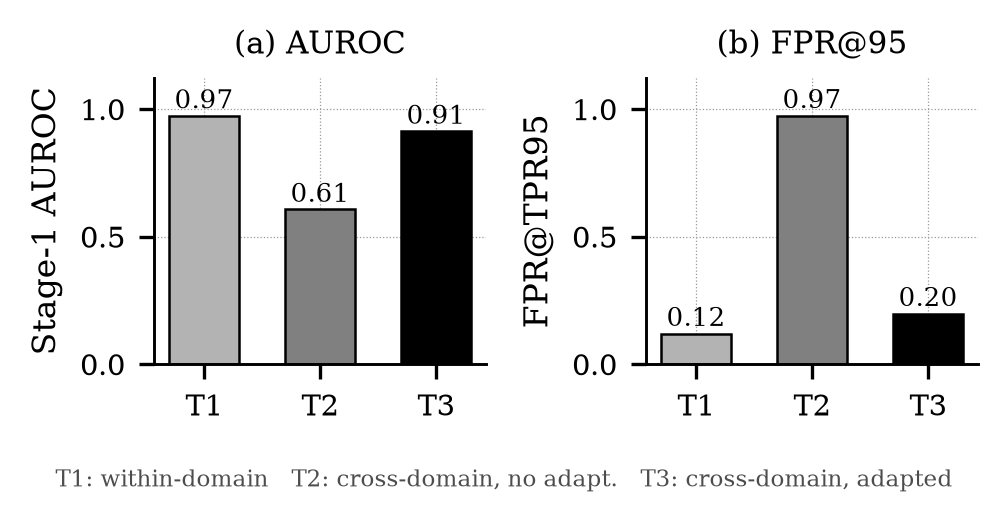
\includegraphics[width=\linewidth]{figures/fig_headline_results.png}
\caption{Sealed-condition Stage-1 AUROC and FPR@TPR95 for the held-out
evaluation (Table~\ref{tab:heldout}).}
\label{fig:headline}
\end{figure}

\subsection{Per-Class Typing}
\label{subsec:perclass}

Table~\ref{tab:perclass} and Figure~\ref{fig:perclass} report per-class
end-to-end F1. Within-domain typing is strong for Benign and Injection
but weak for Recon; Backdoor collapses to $0.000$ within-domain. This is
a direct, concrete instance of the decision-boundary instability
discussed in Section~\ref{subsec:episode_results}: the corrected
entanglement pairs assign Backdoor flows a systematically low Stage-1
attack score, so most Backdoor flows are classified as benign before ever
reaching Stage~2 -- a threshold-placement failure, not a Stage~2 typing
failure. Under cross-domain transfer, attack-type F1 collapses across all
four attack categories. This is a central result rather than a minor
limitation: Q-ARMOR currently adapts binary detection, not the complete
Detect$\to$Type pipeline.

\begin{table*}[t]
\centering
\caption{Current per-class end-to-end F1.}
\label{tab:perclass}
\renewcommand{\arraystretch}{1.1}
\begin{tabular}{@{}lccccc@{}}
\toprule
\textbf{Condition} & \textbf{Benign} & \textbf{DoS} & \textbf{Injection}
                   & \textbf{Recon} & \textbf{Backdoor} \\
\midrule
T1 Within            & 0.949 & 0.590 & 0.830 & 0.112 & 0.000 \\
T3 Cross + S1 adapt  & 0.694 & 0.000 & 0.046 & 0.000 & 0.049 \\
\bottomrule
\end{tabular}
\end{table*}

\begin{figure}[t]
\centering
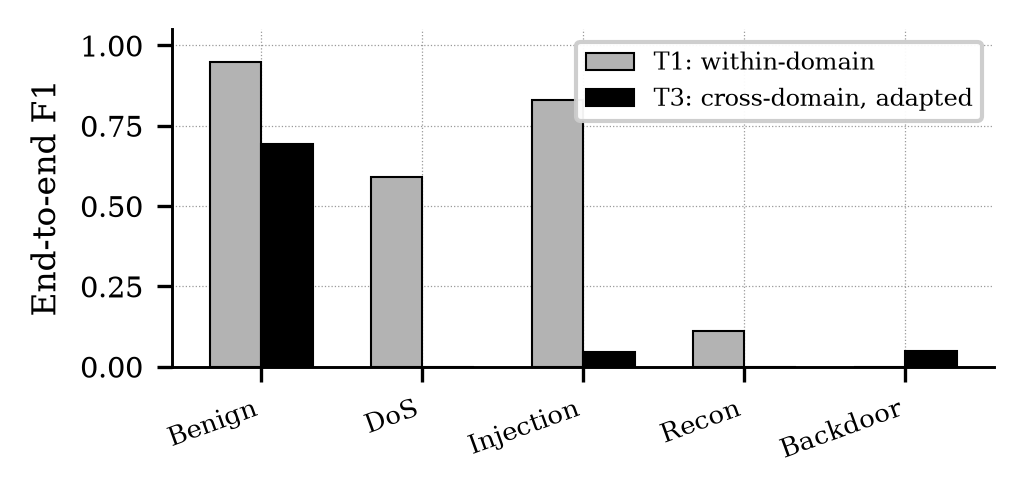
\includegraphics[width=\linewidth]{figures/fig_perclass_typing.png}
\caption{Per-class end-to-end F1, within-domain (T1) versus cross-domain
after Stage-1-only adaptation (T3). Stage-2 typing does not transfer.}
\label{fig:perclass}
\end{figure}

\subsection{LLM-Gated Reflexive Decision Function: Pilot Comparison}
\label{subsec:llm_results}

We ran the identical 10-episode simulation of
Section~\ref{subsec:episode_results} (same fixed QSVC and RF checkpoints,
same episode sampling) under three reflector configurations: the
\textbf{LLM Agent} of Section~\ref{subsec:llm_pilot}, the
\textbf{Rule-based} heuristic SelfReflector, and an \textbf{ADWIN-only}
ablation that fires \textsc{Switch-Subset} whenever ADWIN detects drift
and takes no other action. Table~\ref{tab:llm} and
Figure~\ref{fig:llmcompare} summarise the outcome. We flag this as a
\emph{single-run pilot}; the deltas
below should not be read as a demonstrated policy-quality difference
without seed repetition.

\begin{table*}[t]
\centering
\caption{Reflector comparison, 10 episodes, mean AUROC. ``All'' averages
every episode; ``Cross'' averages Block~B only.}
\label{tab:llm}
\renewcommand{\arraystretch}{1.1}
\begin{tabular}{@{}lccl@{}}
\toprule
\textbf{Reflector} & \textbf{AUROC (all)} & \textbf{AUROC (cross)} &
\textbf{Actions fired} \\
\midrule
LLM Agent   & 0.815 & 0.653 & \textsc{Calibrate-Threshold}$\times8$, \textsc{Switch-Model}$\times2$ \\
Rule-based  & 0.806 & 0.636 & \textsc{Reinforce}$\times3$, \textsc{Switch-Subset}$\times1$, \textsc{Switch-Model}$\times4$ \\
ADWIN-only  & 0.815 & 0.653 & \textsc{Switch-Subset}$\times1$ \\
\bottomrule
\end{tabular}
\end{table*}

\begin{figure}[t]
\centering
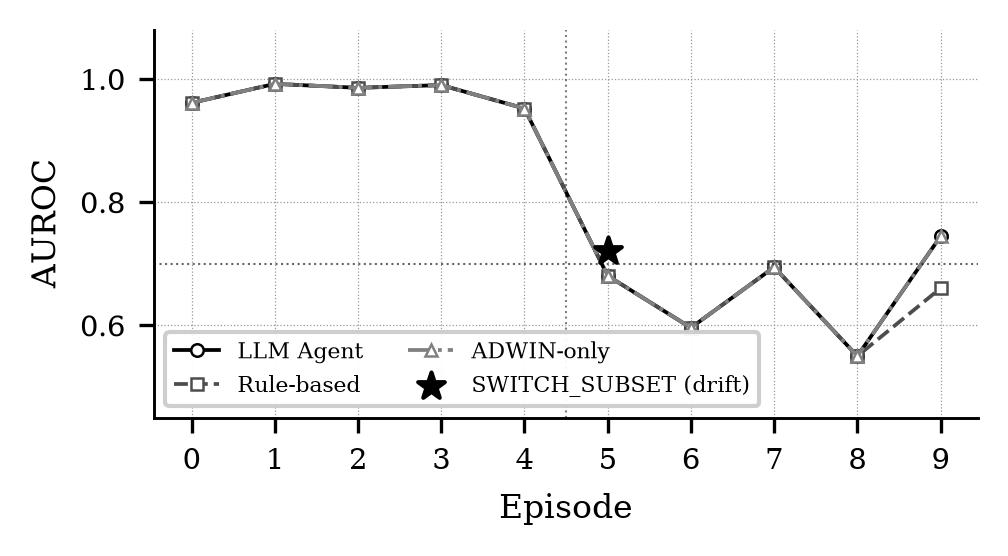
\includegraphics[width=\linewidth]{figures/fig_phase9_comparison.png}
\caption{Episode AUROC under the three reflector configurations. The
star marks episode~5, where ADWIN confirms drift and the Rule-based and
ADWIN-only reflectors fire \textsc{Switch-Subset} -- in contrast to the
independent run of Table~\ref{tab:episodes}, underscoring that drift
confirmation depends on the precise per-sample error sequence.}
\label{fig:llmcompare}
\end{figure}

Three observations, reported with the caveats they warrant. First, in
every episode where FPR@95 was elevated despite acceptable AUROC, the
Diagnoser correctly identified poor decision-boundary placement and the
Planner selected \textsc{Calibrate-Threshold} -- precisely the
threshold-versus-ranking distinction of
Section~\ref{subsec:episode_results}. However, the current evaluation
harness computes hard predictions independently of the policy's decision
threshold, so \textsc{Calibrate-Threshold}'s selection here demonstrates
correct \emph{diagnosis} but not yet a measured \emph{remedial effect}:
the LLM Agent's and ADWIN-only's per-episode AUROC values are identical,
because the action altered no measured outcome in this harness. Second,
the LLM Agent's more conservative exploration -- preferring
\textsc{Calibrate-Threshold} over \textsc{Switch-Model} when both
conditions were technically satisfiable -- resulted in fewer model
demotions and a higher episode-9 AUROC ($0.744$ vs.\ $0.660$ for the
Rule-based reflector, which had already fallen back to Random Forest).
This is a single realisation of a stochastic system, not evidence of
better reasoning in general. Third, \textsc{Switch-Type} was never
triggered: its precondition (Stage-2 macro-F1 collapsing under
cross-domain deployment) is not observable in this binary-only episode
harness, which does not track Stage-2 typing metrics -- \textsc{Switch-Type}
exercised end-to-end remains open future work.

\subsection{Confirmatory Protocol: Equal-Budget Sweep}
\label{subsec:budgetsweep}

Section~\ref{subsec:confirmatory} states that no quantum-superiority
conclusion is valid without comparing quantum and classical adaptation
under the same target-label budget. We ran that comparison: PegasosQSVC
against linear SVM, RBF-SVM, Random Forest, and gradient-boosted trees
(GBT), each retrained from scratch on a target-domain budget
$B \in \{0,25,50,100,150,300\}$ (Eq.~\eqref{eq:budgets}) and evaluated on
the same shared 300-sample cross-domain subset. $B{=}0$ is a fixed
source-only baseline (150-sample source subset, no target data). Classical
models used 10 seeds per $B$; PegasosQSVC used 5, since a single
$(B,\text{seed})$ retrain-and-evaluate cycle costs 15--90 minutes of local
quantum-kernel computation versus under a second for any classical model
-- a cost asymmetry that is itself part of the confirmatory record, not
merely an implementation detail.

\begin{table*}[t]
\centering
\caption{Cross-domain AUROC (mean$\pm$std) versus target-label budget $B$.
Quantum: 5 seeds. Classical: 10 seeds.}
\label{tab:budgetsweep}
\renewcommand{\arraystretch}{1.1}
\begin{tabular}{@{}lcccccc@{}}
\toprule
\textbf{Model} & $B{=}0$ & $B{=}25$ & $B{=}50$ & $B{=}100$ & $B{=}150$ & $B{=}300$ \\
\midrule
PegasosQSVC (quantum) & 0.658 & 0.929$\pm$.012 & 0.902$\pm$.015 & 0.906$\pm$.008 & 0.909$\pm$.009 & 0.909$\pm$.008 \\
Random Forest         & 0.537 & 0.937$\pm$.028 & 0.957$\pm$.019 & 0.978$\pm$.006 & \textbf{0.984$\pm$.003} & \textbf{0.988$\pm$.002} \\
GBT                   & 0.482 & 0.860$\pm$.071 & 0.925$\pm$.033 & 0.969$\pm$.010 & 0.975$\pm$.007 & 0.984$\pm$.003 \\
Linear SVM            & 0.540 & 0.921$\pm$.011 & 0.930$\pm$.011 & 0.941$\pm$.004 & 0.943$\pm$.004 & 0.946$\pm$.003 \\
RBF-SVM               & 0.559 & 0.890$\pm$.038 & 0.928$\pm$.022 & 0.943$\pm$.016 & 0.946$\pm$.011 & 0.949$\pm$.011 \\
\bottomrule
\end{tabular}
\end{table*}

\begin{figure}[t]
\centering
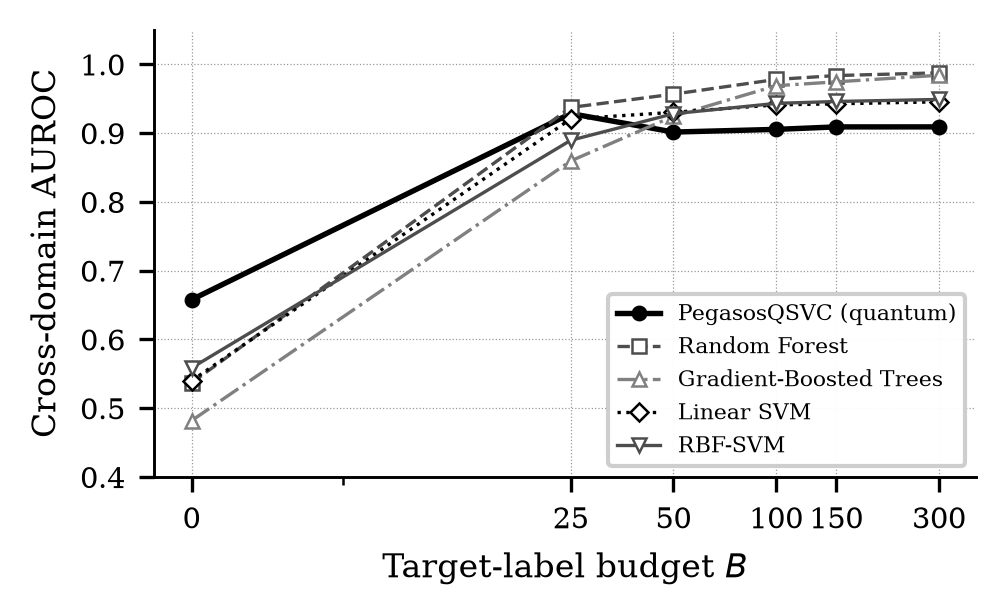
\includegraphics[width=\linewidth]{figures/fig_budget_sweep.png}
\caption{Cross-domain AUROC vs.\ target-label budget $B$ (log-scaled
axis below $B{=}25$). PegasosQSVC leads at very low budgets but plateaus
by $B{=}50$; Random Forest and GBT overtake it from $B{=}100$ onward.}
\label{fig:budgetsweep}
\end{figure}

Table~\ref{tab:budgetsweep} and Figure~\ref{fig:budgetsweep} give a
direct answer: at $B{=}150$, the budget used for this paper's own
headline \textsc{Switch-Subset} result ($T3$, AUROC $0.913$ in
Table~\ref{tab:heldout}), Random Forest reaches $0.984\pm0.003$ and GBT
$0.975\pm0.007$ under the identical protocol -- both above the quantum
kernel's $0.909\pm0.009$, and with roughly one-third the seed-to-seed
variance. At $B{=}300$ the gap widens further (Random Forest
$0.988$ vs.\ PegasosQSVC $0.909$, essentially unchanged from $B{=}150$;
the quantum kernel's AUROC plateaus while every classical baseline
continues to improve with more target data). PegasosQSVC's binary F1 is
also markedly less stable than the classical baselines' at matched
budgets: at $B{=}150$ its F1 standard deviation across seeds is
$0.305$ (mean $0.602$) versus Random Forest's $0.011$ (mean $0.951$),
meaning individual PegasosQSVC retrains at this budget sometimes
collapse to a near-degenerate hard-decision boundary even though AUROC
(a ranking metric, insensitive to threshold placement) stays high --
the same score-orientation sensitivity documented in
Section~\ref{subsec:audit_status}. The one regime where the quantum
kernel visibly leads is the smallest budgets ($B\le25$), consistent with
a compact, structured feature map extracting more signal than an
under-fit classical model can from very little target data; that
advantage does not persist as $B$ grows. \textbf{Table~\ref{tab:budgetsweep}
is therefore direct evidence against, not for, a quantum-superiority
reading of this paper's own $T2\to T3$ recovery}: an equal-budget
classical adaptation would have recovered at least as much cross-domain
AUROC, and more reliably.

\subsection{Confirmatory Protocol: Natural Class Prevalence}
\label{subsec:naturalprev}

Every other evaluation in this paper samples 50/50 balanced flows.
Section~\ref{subsec:confirmatory} requires evaluating natural class
prevalence instead. We re-ran $T1$/$T2$/$T3$ on unbalanced samples
preserving each dataset's true attack rate (ToN-IoT $\approx80\%$,
UNSW-NB15 $\approx3$--$5\%$; PegasosQSVC used a smaller 200-sample draw
for the same compute-cost reason as Section~\ref{subsec:budgetsweep}) and
report the required extra metrics in Table~\ref{tab:naturalprev}:
precision, MCC, balanced accuracy, TPR at FPR${=}0.01$, 10-bin expected
calibration error (ECE), and alerts per 10,000 flows.

\begin{table*}[t]
\centering
\caption{Natural-prevalence $T3$ (cross-domain, adapted) results. Contrast
with the balanced-sample $T3$ row of Table~\ref{tab:heldout}.}
\label{tab:naturalprev}
\renewcommand{\arraystretch}{1.1}
\begin{tabular}{@{}lcccccc@{}}
\toprule
\textbf{Model} & \textbf{AUROC} & \textbf{F1} & \textbf{MCC} & \textbf{Bal.\ Acc.} & \textbf{ECE} & \textbf{Alerts/10k} \\
\midrule
PegasosQSVC (quantum) & 0.849 & 0.137 & 0.200 & 0.772 & 0.349 & 4750 \\
Random Forest         & 0.989 & 0.683 & 0.688 & 0.939 & 0.051 & 790 \\
GBT                   & 0.982 & 0.554 & 0.580 & 0.932 & 0.047 & 1120 \\
Linear SVM            & 0.948 & 0.359 & 0.415 & 0.895 & 0.049 & 2040 \\
RBF-SVM               & 0.944 & 0.361 & 0.413 & 0.888 & 0.083 & 1970 \\
\bottomrule
\end{tabular}
\end{table*}

Two findings, both invisible in the balanced-sample results this paper
otherwise reports. First, binary F1 collapses under true prevalence even
where AUROC stays high: Random Forest's balanced-sample $T3$ F1 is
$0.951$ (Table~\ref{tab:budgetsweep}, $B{=}150$) but falls to $0.683$
under natural prevalence at essentially unchanged AUROC ($0.984\to0.989$)
-- a ranking metric and a threshold metric telling different stories once
the class balance an operator would actually see is restored. Second,
PegasosQSVC's natural-prevalence calibration is the worst of the five
models by a wide margin (ECE $0.349$ vs.\ $0.047$--$0.083$ for every
classical baseline) and its alert rate is the highest (4750 per 10,000
flows, roughly $4$--$6\times$ every classical model's), meaning that at
true prevalence a security operator using the quantum detector would see
far more alerts of far less reliable confidence than with any classical
alternative at the same target-label budget.

\subsection{Confirmatory Protocol: Kernel Diagnostics and Real-QPU Characterisation}
\label{subsec:kerneldiag}

For the quantum-specific diagnostics of Section~\ref{subsec:kta_geo}, we
computed the full $8\times8$-qubit kernel Gram matrix on a fixed
$n{=}100$ balanced source sample, alongside a same-data RBF kernel as
the classical reference. Kernel-target alignment
(Eq.~\eqref{eq:kta}) is $0.353$ for the quantum kernel versus $0.160$ for
RBF -- more than double -- and within-class similarity ($0.250$) exceeds
between-class similarity ($0.049$) by a factor of five, both consistent
with a kernel that induces task-relevant structure rather than an
arbitrary embedding. Effective rank (Eq.~\eqref{eq:reff}) is
$20.5$ out of $100$, indicating the kernel concentrates variance in a
modest number of effective dimensions rather than collapsing to
near-rank-1 or remaining full-rank. The Huang et al.\ geometric
difference \cite{huang2021} is asymmetric: $g(\text{classical}\,\|\,
\text{quantum})=4.86$ versus $g(\text{quantum}\,\|\,\text{classical})=3.39$
(regularisation $\lambda=10^{-3}n$, our own choice, not the original
paper's exact hyperparameter). A geometric difference this size in the
classical-cannot-easily-represent-quantum direction is a
\emph{necessary, not sufficient}, condition for a quantum-kernel
advantage -- it says the quantum kernel induces structure the classical
RBF kernel does not easily reproduce, not that this structure is useful
for this task, a distinction Section~\ref{subsec:budgetsweep} already
answers empirically in the negative for cross-domain AUROC at moderate
and large $B$.

For real-hardware characterisation, we ran a deliberately minimal
6-pair kernel computation (not a full train/evaluate cycle) on
\texttt{ibm\_fez} (156-qubit Heron r2, IBM Quantum Platform, Open plan),
transpiled to the backend's native ISA gate set
(\texttt{generate\_preset\_pass\_manager}) since IBM's runtime primitives
reject un-transpiled circuits. Transpiled depth was 36 with 10 two-qubit
(\texttt{cz}) gates at 1024 shots; wall time including queue was
$65.2\,\text{s}$, of which $4\,\text{s}$ was billed quantum-processor
time -- $0.67\%$ of the Open plan's 600-second (10-minute) monthly
allowance for the entire real-QPU characterisation requirement of
Section~\ref{subsec:confirmatory}. Mean absolute kernel error against the
exact simulator was $0.009$ (max $0.045$) across the six pairs,
consistent with ordinary two-qubit gate and readout noise on current
superconducting hardware and small enough not to change any pair's
qualitative similarity ranking.

\subsection{Confirmatory Protocol: Recurring Domain Shift and Adaptation-Pool Poisoning}
\label{subsec:recurpoison}

\textbf{Recurring drift.} Section~\ref{subsec:confirmatory} asks whether
episodic memory measurably helps beyond a memoryless trigger when a
domain recurs. We ran a 15-episode $A_1\!\to\!B\!\to\!A_2$ stream (5
episodes each; $A{=}$ToN-IoT, $B{=}$UNSW-NB15) under two conditions that
differ in exactly one mechanism: a \emph{persistent} SelfReflector (the
default behaviour reported everywhere else in this paper) and a
\emph{memoryless} ablation that wipes episode \emph{history} -- not
policy state -- at each block transition, so \textsc{Reinforce}'s
3-consecutive-healthy-episode check can never carry across a domain
change. Both conditions fired their first \textsc{Reinforce} in block
$A_2$ at the identical episode (episode 12, the third episode back in the
$A$ domain). This is a negative result reported honestly: because
\textsc{Reinforce} only inspects the two most recent prior episodes
(Section~\ref{subsec:reflexive}), a $>\!2$-episode domain excursion
resets its local streak regardless of whether history persists or is
wiped, so the rule-based reflector's episodic memory provides \emph{no
measurable benefit} across this recurrence gap. This is precisely the
gap the LLM-gated pilot's RAG-based semantic-memory retrieval
(Section~\ref{subsec:llm_pilot}) was designed to address, since it
retrieves over the \emph{full} episode history rather than a
fixed 2-episode window; a multi-seed reflector comparison remains open
(Section~\ref{subsec:llm_results}), so this remains a motivated design
distinction rather than a demonstrated one.

\textbf{Poisoning.} We flipped a controlled fraction
(0--50\%) of ATTACK-labelled rows to BENIGN in the \textsc{Switch-Subset}
adaptation pool before retraining -- an attacker hiding traffic from the
next retrain, matching the Threat Model of
Section~\ref{subsec:threat} -- for PegasosQSVC, Random Forest, and GBT,
then evaluated on the clean (never-poisoned) test split and probed
whether \textsc{Reinforce} would fire on the resulting model.

\begin{figure}[t]
\centering
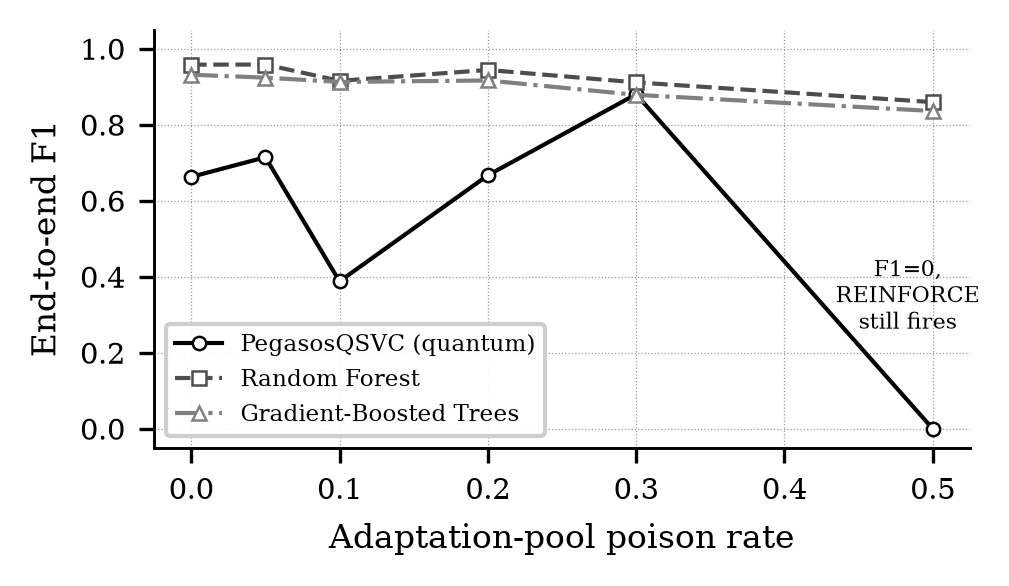
\includegraphics[width=\linewidth]{figures/fig_poisoning.png}
\caption{End-to-end F1 on the clean test set vs.\ adaptation-pool poison
rate. \textsc{Reinforce} fires at every rate for every model shown,
including where PegasosQSVC's F1 collapses to 0 at 50\% poisoning.}
\label{fig:poisoning}
\end{figure}

Figure~\ref{fig:poisoning} shows the result: \textsc{Reinforce} fired at
\emph{every} poison rate for \emph{every}
model tested, with no exception. The starkest case is PegasosQSVC at
50\% poisoning: AUROC stays at $0.909$ (statistically indistinguishable
from the clean-pool value) while F1 collapses to exactly $0.000$ --
the retrained decision boundary stops making a single correct positive
prediction on the clean test set, yet \textsc{Reinforce} still fires,
because its rule inspects only AUROC, never F1, precision, or recall.
Random Forest and GBT degrade far more gracefully over the same range
(F1 falling from $0.958\to0.859$ and $0.932\to0.836$ respectively) but
\textsc{Reinforce} fires identically regardless. This is a direct,
measured confirmation of the limitation the Threat Model already states
on structural grounds: \emph{the persistent controller has no built-in
poisoning defence}, and can lock in an adaptation-pool-poisoned model as
confidently as a clean one.

% ============================================================
\section{Analysis and Discussion}
\label{sec:discussion}
% ============================================================

\subsection{What the Current Evidence Establishes}

The present experiments establish three narrow points. First, an 8-qubit
fidelity kernel trained on a small representative source subset can
produce useful within-domain binary discrimination in the reported run.
Second, a substantial source$\to$target degradation occurs between the
two NetFlow corpora. Third, replacing the source kernel subset with 150
representative labelled target flows recovers part of the lost binary
performance. The LLM-gated pilot of Section~\ref{subsec:llm_results}
adds a fourth, narrower point: an inference-time language-reasoning
decision function, gated by a deterministic verifier, can reproduce the
rule-based controller's core triage behaviour while additionally
surfacing a threshold-placement failure mode the rule-based reflector
has no mechanism to diagnose.

The confirmatory protocol of Section~\ref{subsec:confirmatory}, run in
full on the first three points above, adds a fifth, corrective point:
the recovery in point three is \emph{not} evidence of quantum advantage
or superior sample efficiency. At the paper's own adaptation budget and
beyond, equal-budget classical baselines match or exceed the quantum
kernel's cross-domain AUROC with substantially lower variance
(Section~\ref{subsec:budgetsweep}), the quantum kernel's calibration
under natural class prevalence is markedly worse than every classical
alternative (Section~\ref{subsec:naturalprev}), and the reflexive
controller -- rule-based or LLM-gated -- has no mechanism to detect
adaptation-pool poisoning regardless of which detector it drives
(Section~\ref{subsec:recurpoison}). The evidence still does not establish
unsupervised drift detection, learned policy improvement (by either
reflector variant), general multi-domain robustness beyond the single
tested pair, or full-scale real-QPU viability beyond the minimal
characterisation of Section~\ref{subsec:kerneldiag}; these remain the
protocol's open items (Section~\ref{subsec:confirmatory}).

\subsection{Quantum Contribution and Required Geometry Diagnostics}
\label{subsec:kta_geo}

The scientific value of the quantum component should be assessed through
its induced geometry, not through rhetoric about high-dimensional Hilbert
spaces. For a Gram matrix $K$ and binary label kernel $Y = \mathbf{y}
\mathbf{y}^{\top}$, centred kernel-target alignment can be measured by
\begin{equation}
\text{KTA}(K,Y) = \frac{\langle K_c, Y_c \rangle_F}{\|K_c\|_F \|Y_c\|_F}.
\label{eq:kta}
\end{equation}
If $\lambda_1,\dots,\lambda_n$ are Gram eigenvalues, an effective-rank
diagnostic is
\begin{equation}
r_{\text{eff}}(K) = \frac{\left(\sum_i \lambda_i\right)^2}{\sum_i
\lambda_i^2}.
\label{eq:reff}
\end{equation}
Together with within/between-class similarity and the classical--quantum
geometric difference proposed by Huang et al.\ \cite{huang2021}, these
quantities can show whether the chosen feature map creates task-relevant
structure or merely an expensive approximation of a classical kernel.
Section~\ref{subsec:kerneldiag} reports all four diagnostics for the
deployed kernel.

\subsection{Why Cross-Domain Typing Fails}

Stage~1 uses a portable binary label space, whereas Stage~2 relies on a
hand-built coarse taxonomy whose semantics differ between datasets.
Consequently, adapting only Stage~1 cannot repair a target-domain type
classifier trained on source attack mechanisms. A stronger design should
use an attack-only Stage~2, introduce an \emph{Unknown} class, and
allocate a separate target-label budget to type adaptation. Open-set
evaluation is preferable to forcing every target attack into a
source-defined category. \textsc{Switch-Type} (Section~\ref{subsec:llm_pilot})
is designed for exactly this purpose but remains untriggered in the
current pilot.

\subsection{Reflexive Control versus Policy Learning}
\label{subsec:policy_learning}

Persistent memory changes what information is available to the
controller, but the current action mapping is fixed in both reflector
variants. Thus the prototype implements autonomous stateful control, not
learning. This holds equally for the rule-based SelfReflector, whose
mapping is a fixed threshold table, and for the LLM-gated reflector of
Section~\ref{subsec:llm_pilot}, whose per-episode output depends on the
language model's reasoning over the same evaluator signals but updates no
parameters from outcomes -- the two variants differ in \emph{how} a
decision is reached, not in \emph{whether} the decision rule adapts from
experience. A genuine learned extension can represent the episode state
as
\begin{equation}
\mathbf{z}_t = [d_t, u_t, c_t, \Delta_t, b_t, \ell_t, m_t],
\label{eq:state}
\end{equation}
where $d_t$ is drift evidence, $u_t$ uncertainty, $c_t$ calibration,
$\Delta_t$ performance trend, $b_t$ remaining budget, $\ell_t$
latency/circuit cost, and $m_t$ memory features. A contextual bandit
could then choose among keep, recalibrate, reselect, retrain, classical
fallback, and abstain actions while optimising Eq.~\eqref{eq:objective}.
Such a model would justify the phrase \emph{policy learning}; the current
manuscript -- for both reflector variants -- deliberately does not claim
it.

\textbf{Operational Interpretation.} The $\approx 3$\,s per-sample
quantum inference latency precludes line-rate deployment. A practical
hybrid architecture therefore uses classical models for real-time
detection and selectively invokes quantum-kernel analysis for batch
assessment, uncertain samples, or adaptation, enabling explicit control
of quantum-computation cost.

\textbf{Limitations.} Current limitations include: (i)~the headline
held-out numbers of Table~\ref{tab:heldout} are still a single run --
score orientation is now verified (Section~\ref{subsec:audit_status}) and
multi-seed statistics exist for the confirmatory budget sweep
(Section~\ref{subsec:budgetsweep}), but have not yet been re-applied to
re-derive Table~\ref{tab:heldout} itself; (ii)~evaluation on only one
source$\to$target transfer pair, since NF-BoT-IoT and
NF-CSE-CIC-IDS2018 are not yet incorporated
(Section~\ref{subsec:confirmatory}); (iii)~dependence on label feedback
for ADWIN and episodic metrics; (iv)~non-adaptive Stage~2 typing;
(v)~real-hardware evidence is now a minimal 6-pair characterisation
(Section~\ref{subsec:kerneldiag}), not a full train/evaluate cycle on
a QPU; (vi)~the LLM-gated pilot's \textsc{Calibrate-Threshold} action
is not yet wired into the prediction path, so its measured effect is
currently null by construction, not by evidence of ineffectiveness; and
(vii)~the LLM pilot itself is a single run with no seed repetition.
Equal-budget classical adaptation and adaptation-pool poisoning are no
longer untested (Sections~\ref{subsec:budgetsweep}
and~\ref{subsec:recurpoison} respectively); both instead now weigh
\emph{against} the quantum kernel's competitiveness and \emph{confirm}
the controller's lack of poisoning defence.

% ============================================================
\section{Conclusion}
\label{sec:conclusion}
% ============================================================

We presented a substantially revised Q-ARMOR as a reflexive quantum-kernel
IDS for cross-domain adaptation. It combines fidelity-kernel binary
detection, classical attack typing, episodic state, and explicit
adaptation actions, executable under either a deterministic rule-based
reflector or a piloted LLM-gated alternative with an identical
deterministic safety gate. Current results show strong within-domain
performance, severe cross-domain degradation, and partial recovery using
150 labelled target flows, while attack typing remains non-transferable
and simulator results do not support hardware claims. The LLM-gated pilot
additionally surfaces a threshold-placement failure mode invisible to the
rule-based reflector, though its remedial mechanism is not yet wired into
measured outcomes. Q-ARMOR is positioned as a study of adaptive
quantum-kernel representation under network domain shift, not as evidence
of quantum advantage or learned autonomous optimisation, by either
reflector variant. Section~\ref{subsec:confirmatory} details, without
exception, the confirmatory work completed and still required before any
stronger claim would be warranted.

% ============================================================
\section*{Acknowledgment}

The authors thank Dr.\ Shiva Raj Pokhrel for supervision and guidance
throughout this research, and the Deakin University HPC team for
computational support.

% ============================================================
\begin{thebibliography}{99}

\bibitem{shinn2023}
N.~Shinn, F.~Cassano, A.~Gopinath, K.~Narasimhan, and S.~Yao,
``Reflexion: Language agents with verbal reinforcement learning,''
\textit{Advances in Neural Information Processing Systems}, vol.~36, 2023.

\bibitem{havlicek2019}
V.~Havl\'{i}\v{c}ek, A.~D.~C\'{o}rcoles, K.~Temme, A.~W.~Harrow,
A.~Kandala, J.~M.~Gambetta, and J.~M.~Chow,
``Supervised learning with quantum-enhanced feature spaces,''
\textit{Nature}, vol.~567, pp.~209--212, 2019.

\bibitem{schuld2019}
M.~Schuld and N.~Killoran,
``Quantum machine learning in feature Hilbert spaces,''
\textit{Physical Review Letters}, vol.~122, no.~4, p.~040504, 2019.

\bibitem{huang2021}
H.-Y.~Huang, M.~Broughton, M.~Mohseni, R.~Babbush, S.~Boixo, H.~Neven,
and J.~R.~McClean,
``Power of data in quantum machine learning,''
\textit{Nature Communications}, vol.~12, Art.\ no.~2631, 2021.

\bibitem{cerezo2022}
M.~Cerezo, G.~Verdon, H.-Y.~Huang, L.~Cincio, and P.~J.~Coles,
``Challenges and opportunities in quantum machine learning,''
\textit{Nature Computational Science}, vol.~2, pp.~567--576, 2022.

\bibitem{thanasilp2024}
S.~Thanasilp, S.~Wang, M.~Cerezo, and Z.~Holmes,
``Exponential concentration in quantum kernel methods,''
\textit{Nature Communications}, vol.~15, Art.\ no.~5200, 2024.

\bibitem{bendavid2010}
S.~Ben-David, J.~Blitzer, K.~Crammer, A.~Kulesza, F.~Pereira, and
J.~W.~Vaughan,
``A theory of learning from different domains,''
\textit{Machine Learning}, vol.~79, pp.~151--175, 2010.

\bibitem{bifet2007}
A.~Bifet and R.~Gavald\`{a},
``Learning from time-changing data with adaptive windowing,''
in \textit{Proc.\ 7th SIAM Int.\ Conf.\ Data Mining (SDM)}, 2007,
pp.~443--448.

\bibitem{liao2013}
H.-J.~Liao, C.-H.~R.~Lin, Y.-C.~Lin, and K.-Y.~Tung,
``Intrusion detection system: A comprehensive review,''
\textit{Journal of Network and Computer Applications},
vol.~36, no.~1, pp.~16--24, 2013.

\bibitem{breiman2001}
L.~Breiman,
``Random forests,''
\textit{Machine Learning}, vol.~45, no.~1, pp.~5--32, 2001.

\bibitem{sarhan2021}
M.~Sarhan, S.~Layeghy, and M.~Portmann,
``Towards a standard feature set for network intrusion detection
system datasets,''
\textit{Mobile Networks and Applications},
vol.~27, no.~1, pp.~357--370, 2022.

\bibitem{toniot}
N.~Moustafa,
``NF-ToN-IoT: A novel dataset for evaluating network traffic
intrusion detection systems,''
\textit{IEEE Access}, vol.~9, pp.~94--106, 2021.

\bibitem{kalinin2022}
M.~Kalinin and V.~Krundyshev,
``Security intrusion detection using quantum machine learning
techniques,''
\textit{Journal of Computer Virology and Hacking Techniques},
vol.~19, pp.~125--136, 2023.

\bibitem{qiskit_ml}
IBM Qiskit Machine Learning Development Team,
\textit{Qiskit Machine Learning}, version~0.9 documentation and
open-source software, 2025--2026. [Online]. Available:
\url{https://qiskit-community.github.io/qiskit-machine-learning/}

\bibitem{llama3}
A.~Grattafiori \textit{et al.},
``The Llama 3 herd of models,''
arXiv preprint arXiv:2407.21783, 2024.

\end{thebibliography}

\end{document}
